\documentclass[11pt,a4paper]{article}

% --- Packages ---
\usepackage[margin=1in]{geometry}
\usepackage{amsmath}
\usepackage{amssymb}
\usepackage{booktabs}
\usepackage{hyperref}
\usepackage{enumitem}
\usepackage{tabularx}
\usepackage{graphicx}
\usepackage{microtype}
\usepackage{setspace}
\usepackage{titlesec}
\usepackage{times}
\usepackage{cite}
\usepackage{float}
\usepackage{multicol}
\usepackage{tikz}
\usetikzlibrary{shapes,arrows,positioning,calc}
\usepackage{multirow}

% Theorem environments
\newtheorem{definition}{Definition}
\newtheorem{proposition}{Proposition}
\newtheorem{hypothesis}{Hypothesis}

\hypersetup{
    colorlinks=true,
    linkcolor=blue,
    citecolor=blue,
    urlcolor=blue
}

\titleformat{\section}{\Large\bfseries}{\thesection}{1em}{}
\titleformat{\subsection}{\large\bfseries}{\thesubsection}{1em}{}
\titleformat{\subsubsection}{\normalsize\bfseries}{\thesubsubsection}{1em}{}

\onehalfspacing

\title{\textbf{The E3 Framework: A Conceptual Framework for Software Quality in the Age of Artificial Intelligence}}
\author{%
    Md. Niaj Shahriar Shishir\\Head of Technology, Metamorphosis Ltd\\
    \texttt{nsrshishir550@gmail.com}
}
\date{\today}

\begin{document}

\maketitle

% ============================================================
% ABSTRACT
% ============================================================
\begin{abstract}
\noindent
The integration of artificial intelligence into mainstream software development has precipitated a paradigm shift from deterministic systems---where outputs are fully predictable given inputs---to probabilistic systems, where outputs are stochastic, context-dependent, and ethically consequential. This transition creates a critical gap: traditional software quality models were designed for deterministic paradigms and struggle to address the unique challenges posed by machine learning systems, large language models, and AI-driven applications. This paper introduces the \textbf{E3 Framework}, a \emph{conceptual framework} organized around three mutually reinforcing pillars: \emph{Effectiveness} ($E_1$: alignment with user needs, ethical imperatives, and SOLID principles), \emph{Efficiency} ($E_2$: computational sustainability, resource optimization, and DRY/KISS principles), and \emph{Elegance} ($E_3$: cognitive accessibility, human-computer interaction excellence, and explainable AI). Formal mathematical definitions are presented for each pillar, along with a trade-off function enabling principled priority-setting and testable hypotheses for future empirical validation. Through comparative analysis with ISO 25010, McCall's quality factors, NIST AI RMF, and the EU AI Act, E3 is demonstrated to synthesize and extend existing quality models with AI-specific concerns: alignment and fairness for effectiveness; computational sustainability for efficiency; and explainability with actionability for elegance. The framework is operationalized through specific metrics with formulas and thresholds, with its application demonstrated through four illustrative hypothetical scenarios across healthcare, recommendation systems, code assistance, and autonomous vehicles. The framework addresses a critical need: preserving the hard-won wisdom of traditional software engineering while extending it to govern probabilistic, AI-driven systems that are simultaneously reliable, sustainable, and humane. The paper concludes with a transparent discussion of validity threats and a research agenda for empirical validation.
\end{abstract}

\noindent\textbf{Keywords:} Software Engineering, Artificial Intelligence, Machine Learning, Software Quality, AI Ethics, Explainable AI, Computational Sustainability, MLOps, Prompt Engineering

\vspace{1em}

% ============================================================
% 1. INTRODUCTION
% ============================================================
\section{Introduction}

\subsection{The Deterministic Foundations of Software Engineering}

For over six decades, software engineering matured under a deterministic paradigm: given identical inputs, a correctly implemented program produces identical outputs. This foundational assumption enabled the development of rigorous methodologies, testing frameworks, and quality assurance practices that transformed software from an artisanal craft into a disciplined engineering profession. Fred Brooks's seminal observation that ``complexity is the essential difficulty of software'' \cite{brooks1975mythical} established the intellectual foundation for decades of research into managing this complexity through abstraction, modularity, and structured design.

The discipline responded with principles that have stood the test of time. Barry Boehm's spiral model \cite{boehm1988spiral} introduced risk-driven iterative development. Kent Beck's Extreme Programming \cite{beck2000extreme} emphasized adaptive planning and continuous improvement. Robert C. Martin's SOLID principles \cite{martin2017clean} provided architectural guidelines that remain cornerstones of object-oriented design. The Pragmatic Programmer philosophy \cite{hunt1999pragmatic} distilled wisdom about DRY (Don't Repeat Yourself), orthogonality, and the importance of writing code that communicates intent. These principles share a common assumption: that software behavior can be specified, verified, and reproduced deterministically.


\subsection{The Rise of Probabilistic Systems}

The emergence of machine learning and artificial intelligence has fundamentally disrupted this equilibrium. A large language model does not guarantee deterministic output; its behavior is shaped by training data distributions, sampling parameters, and prompt context. As Brown et al. demonstrated with GPT-3 \cite{brown2020language}, a single model can exhibit remarkable few-shot learning capabilities across diverse tasks, yet produce outputs that vary between invocations even with identical inputs. This stochastic nature represents not a bug but a fundamental architectural difference.

Sculley et al. documented the profound implications of this shift in their influential paper on technical debt in machine learning systems \cite{sculley2015hidden}. They identified unique challenges that classical design patterns were never intended to address: ``pipeline jungles'' created by ad-hoc data transformations, ``entanglement'' where changing any input feature affects all predictions, and ``hidden feedback loops'' where models influence their own training data. Amershi et al. extended this analysis through empirical studies at Microsoft \cite{amershi2019software}, finding that ML-enabled systems require fundamentally different engineering practices across data management, model versioning, and deployment pipelines.

The implications extend beyond technical architecture. Russell \cite{russell2019human} argued that the alignment problem---ensuring AI systems pursue objectives that genuinely reflect human intent---represents a core challenge distinct from traditional correctness criteria. A recommendation system may be technically accurate while systematically discriminating against protected groups. A language model may generate fluent prose while hallucinating false information. The very notion of ``correctness'' becomes contested in probabilistic systems.

\subsection{The Gap: Traditional Methodologies Meet AI Challenges}

Existing software development methodologies address fragments of this transition but lack a unified quality model spanning both classical and AI-driven development. Agile methodologies excel at iterative delivery and customer feedback but provide limited guidance for managing model uncertainty or ensuring fairness \cite{beck2000extreme}. DevOps practices automate deployment pipelines but were designed for deterministic services where integration tests can verify behavior \cite{humble2010continuous}. MLOps extends DevOps for machine learning but often treats ethical considerations and explainability as secondary concerns \cite{sridhar2022mlops}.

This paper introduces the E3 Framework as a response to this methodological gap. Rather than discarding the hard-won principles of traditional software engineering, E3 extends them into the probabilistic domain through three mutually reinforcing pillars:

\begin{enumerate}[leftmargin=2em]
    \item \textbf{Effectiveness ($E_1$)}---software that solves the right problem, for the right people, within ethical boundaries.
    \item \textbf{Efficiency ($E_2$)}---software that minimizes waste in computation, code, and cognition.
    \item \textbf{Elegance ($E_3$)}---software that is cognitively accessible, aesthetically coherent, and transparently explainable.
\end{enumerate}

\subsection{Paper Organization and Contributions}

This paper makes the following contributions:

\begin{enumerate}[leftmargin=2em]
    \item \textbf{Formal Definitions:} We provide mathematically precise definitions for each E3 pillar, enabling rigorous reasoning about software quality (Section~\ref{sec:formal_definitions}).
    \item \textbf{Comparative Analysis:} We position E3 relative to established quality models (ISO 25010, McCall) and AI governance frameworks (NIST AI RMF, EU AI Act), demonstrating both continuity and extensions (Section~\ref{sec:related_work}).
    \item \textbf{Metrics Operationalization:} We define specific, measurable metrics for each pillar with formulas, target thresholds, and collection methodologies (Section~\ref{sec:metrics_operationalization}).
    \item \textbf{Illustrative Examples:} We demonstrate framework application through four hypothetical scenarios across diverse domains (Section~\ref{sec:illustrative_examples}).
    \item \textbf{Validity Analysis:} We transparently address threats to validity and propose a research agenda for empirical validation (Section~\ref{sec:threats_to_validity}).
\end{enumerate}

We explicitly position E3 as a \emph{conceptual framework}---a structured way of thinking about software quality that generates testable hypotheses---rather than a validated methodology. This positioning is honest about the framework's current status while providing a foundation for future empirical research.

% ============================================================
% 2. FORMAL DEFINITIONS AND THEORETICAL FOUNDATIONS
% ============================================================
% ============================================================
% FORMAL DEFINITIONS AND THEORETICAL FOUNDATIONS
% ============================================================

\section{Formal Definitions and Theoretical Foundations}
\label{sec:formal_definitions}

This section presents the formal mathematical foundations of the E3 Framework, providing rigorous definitions that enable precise reasoning about software quality in both deterministic and probabilistic systems. These definitions establish the theoretical basis for the framework's three pillars and their interrelationships.

\subsection{The E3 Quality Space}

\begin{definition}[E3 Quality Vector]
\label{def:quality_vector}
Let $\mathcal{Q}$ denote the \emph{E3 Quality Space}, defined as a bounded three-dimensional vector space:

\begin{equation}
\mathcal{Q} = \left\{ \mathbf{q} = (E_1, E_2, E_3) \in \mathbb{R}^3 \mid 0 \leq E_i \leq 1, \; i \in \{1, 2, 3\} \right\}
\end{equation}

where each component represents a normalized quality dimension:
\begin{itemize}[leftmargin=2em]
    \item $E_1 \in [0,1]$: \textbf{Effectiveness score} --- degree to which the software fulfills stakeholder requirements within ethical boundaries
    \item $E_2 \in [0,1]$: \textbf{Efficiency score} --- ratio of value delivered to resources consumed across computational, cognitive, and financial dimensions
    \item $E_3 \in [0,1]$: \textbf{Elegance score} --- degree to which the software is cognitively accessible, transparently explainable, and aesthetically coherent
\end{itemize}
\end{definition}

The normalization to $[0,1]$ enables comparison across heterogeneous systems and provides a foundation for aggregation and trade-off analysis.

\subsection{Formal Pillar Definitions}

\subsubsection{Effectiveness (\texorpdfstring{$E_1$}{E1})}

\begin{definition}[Effectiveness]
\label{def:effectiveness}
Effectiveness $E_1$ is defined as the conjunction of functional correctness and ethical compliance:

\begin{equation}
E_1 = \alpha \cdot F(S) + (1 - \alpha) \cdot C(S)
\end{equation}

where:
\begin{itemize}[leftmargin=2em]
    \item $F(S) \in [0,1]$ is the \emph{functional correctness} of system $S$, measuring the degree to which outputs satisfy specified requirements
    \item $C(S) \in [0,1]$ is the \emph{ethical compliance} of system $S$, measuring adherence to fairness constraints, transparency requirements, and governance standards
    \item $\alpha \in [0,1]$ is a domain-specific weighting parameter reflecting the relative importance of functional versus ethical considerations
\end{itemize}

For AI systems, functional correctness extends beyond traditional correctness to include:

\begin{equation}
F(S_{AI}) = \beta_1 \cdot \text{Accuracy} + \beta_2 \cdot \text{Robustness} + \beta_3 \cdot \text{Alignment}
\end{equation}

where Alignment measures the correspondence between system behavior and genuine stakeholder intent \cite{russell2019human}.
\end{definition}

\subsubsection{Efficiency (\texorpdfstring{$E_2$}{E2})}

\begin{definition}[Efficiency]
\label{def:efficiency}
Efficiency $E_2$ is defined as the ratio of value delivered to total resources consumed:

\begin{equation}
E_2 = \frac{V(S)}{R_{compute}(S) + R_{carbon}(S) + R_{cognitive}(S) + R_{financial}(S)}
\end{equation}

where:
\begin{itemize}[leftmargin=2em]
    \item $V(S)$ represents the value delivered by system $S$ (measured through stakeholder-defined metrics)
    \item $R_{compute}(S)$ represents computational resource consumption (FLOPs, memory, latency)
    \item $R_{carbon}(S)$ represents environmental impact (carbon emissions, energy consumption) \cite{strubell2019energy, patterson2021carbon}
    \item $R_{cognitive}(S)$ represents developer and user cognitive effort
    \item $R_{financial}(S)$ represents monetary costs (infrastructure, API calls, maintenance)
\end{itemize}

For LLM-based systems, efficiency includes token economics:

\begin{equation}
E_2^{LLM} = \frac{\text{Quality per Query}}{\text{Tokens}_{prompt} + \text{Tokens}_{completion}} \cdot \frac{1}{\text{Retry Rate}}
\end{equation}
\end{definition}

\subsubsection{Elegance (\texorpdfstring{$E_3$}{E3})}

\begin{definition}[Elegance]
\label{def:elegance}
Elegance $E_3$ is defined as the geometric mean of cognitive accessibility, explainability, and aesthetic integrity:

\begin{equation}
E_3 = \sqrt[3]{U(S) \cdot X(S) \cdot A(S)}
\end{equation}

where:
\begin{itemize}[leftmargin=2em]
    \item $U(S) \in [0,1]$ is \emph{usability}, measuring cognitive accessibility per Nielsen's heuristics \cite{nielsen1994enhancing} and ISO 9241-210 \cite{iso2019ergonomics}
    \item $X(S) \in [0,1]$ is \emph{explainability}, measuring the degree to which system reasoning is transparent to stakeholders \cite{doshivelez2017towards, ribeiro2016should}
    \item $A(S) \in [0,1]$ is \emph{aesthetic integrity}, measuring coherence between form and function
\end{itemize}

For AI systems, explainability decomposes as:

\begin{equation}
X(S_{AI}) = \gamma_1 \cdot \text{Interpretability} + \gamma_2 \cdot \text{Transparency} + \gamma_3 \cdot \text{Actionability}
\end{equation}

where Actionability measures whether explanations enable users to effectively correct or refine system outputs.
\end{definition}

\subsection{Trade-off Function}

\begin{definition}[E3 Trade-off Function]
\label{def:tradeoff}
The E3 Trade-off Function $T: \mathcal{Q} \rightarrow [0,1]$ aggregates quality dimensions according to stakeholder priorities:

\begin{equation}
T(\mathbf{q}) = w_1 E_1 + w_2 E_2 + w_3 E_3
\end{equation}

subject to constraints:
\begin{equation}
\sum_{i=1}^{3} w_i = 1, \quad w_i \geq 0 \quad \forall i \in \{1, 2, 3\}
\end{equation}

The weight vector $\mathbf{w} = (w_1, w_2, w_3)$ encodes domain-specific priorities:
\begin{itemize}[leftmargin=2em]
    \item \textbf{Safety-critical systems} (healthcare, autonomous vehicles): $\mathbf{w} \approx (0.6, 0.2, 0.2)$
    \item \textbf{High-volume systems} (content recommendation, ad targeting): $\mathbf{w} \approx (0.3, 0.5, 0.2)$
    \item \textbf{User-facing creative tools} (design assistants, writing tools): $\mathbf{w} \approx (0.3, 0.2, 0.5)$
\end{itemize}
\end{definition}

\subsection{Theoretical Propositions}

The following propositions establish theoretical relationships within the E3 Framework that can be empirically tested in future research.

\begin{proposition}[Pillar Interdependence]
\label{prop:interdependence}
For any software system $S$, the three quality pillars are not independent. Specifically:

\begin{enumerate}[leftmargin=2em]
    \item \textbf{Effectiveness-Efficiency Trade-off:} $\frac{\partial E_1}{\partial E_2} \leq 0$ in the region of high effectiveness, indicating diminishing returns where further effectiveness gains require disproportionate efficiency costs.
    
    \item \textbf{Effectiveness-Elegance Trade-off:} Complex models achieving high $E_1$ often exhibit low $X(S)$, suggesting $\text{Corr}(E_1, E_3) < 0$ for certain model classes.
    
    \item \textbf{Efficiency-Elegance Synergy:} Well-designed abstractions that improve elegance (clean interfaces, modular design) often improve efficiency through reduced cognitive load and maintenance cost, suggesting $\text{Corr}(E_2, E_3) > 0$ for well-architected systems.
\end{enumerate}
\end{proposition}

\begin{proposition}[Pareto Optimality]
\label{prop:pareto}
For a given weight vector $\mathbf{w}$, an optimal system $S^*$ satisfies:

\begin{equation}
S^* = \arg\max_{S} T(\mathbf{q}(S))
\end{equation}

subject to minimum thresholds:
\begin{equation}
E_i(S) \geq \tau_i \quad \forall i \in \{1, 2, 3\}
\end{equation}

where $\tau_i$ represents domain-specific minimum acceptable quality for each pillar.
\end{proposition}

\begin{proposition}[AI Transition Discontinuity]
\label{prop:transition}
The transition from deterministic to probabilistic systems introduces a discontinuity in the effectiveness measurement function:

\begin{equation}
\lim_{\sigma \rightarrow 0} F(S_{probabilistic}) \neq F(S_{deterministic})
\end{equation}

where $\sigma$ represents output variance. This discontinuity necessitates the extended definitions of effectiveness (including alignment) and elegance (including explainability) for AI systems.
\end{proposition}

\subsection{Testable Hypotheses}

The following hypotheses operationalize the theoretical framework for empirical validation:

\begin{hypothesis}[H1: Framework Adoption Impact]
\label{hyp:adoption}
Teams explicitly using the E3 Framework will produce systems with measurably higher trade-off scores $T(\mathbf{q})$ compared to teams using ad-hoc quality approaches, controlling for team experience and project complexity.
\end{hypothesis}

\begin{hypothesis}[H2: Trade-off Awareness]
\label{hyp:awareness}
Explicit articulation of weight vector $\mathbf{w}$ during requirements gathering reduces post-deployment quality disputes by enabling stakeholder alignment on priorities.
\end{hypothesis}

\begin{hypothesis}[H3: Pillar Coverage]
\label{hyp:coverage}
Existing software quality models (ISO 25010, McCall) provide incomplete coverage of the E3 quality space for AI systems, specifically lacking explicit representation of:
\begin{itemize}[leftmargin=2em]
    \item Alignment as a component of effectiveness
    \item Carbon footprint as a component of efficiency
    \item Explainability as a component of elegance
\end{itemize}
\end{hypothesis}

\begin{hypothesis}[H4: Prompt Engineering Validity]
\label{hyp:prompt}
For LLM-based systems, E3-based prompt evaluation correlates positively with downstream task performance and user satisfaction, providing a predictive quality signal during development.
\end{hypothesis}

\subsection{Relationship to Existing Quality Models}

Table~\ref{tab:quality_model_mapping} maps E3 components to established quality models, demonstrating both continuity with traditional software engineering and extensions for AI systems.

\begin{table*}[t]
\centering
\caption{Mapping E3 Pillars to Existing Quality Models}
\label{tab:quality_model_mapping}
\small
\begin{tabularx}{\textwidth}{@{}l X X X@{}}
\toprule
\textbf{Quality Model} & \textbf{$E_1$ (Effectiveness)} & \textbf{$E_2$ (Efficiency)} & \textbf{$E_3$ (Elegance)} \\
\midrule
ISO 25010 \cite{iso25010:2011} & Functional Suitability, Reliability, Security & Performance Efficiency & Usability \\
McCall \cite{mccall1977factors} & Correctness, Integrity, Reliability & Efficiency & Usability \\
Boehm \cite{boehm1978characteristics} & Functionality, Reliability & Efficiency, Economy & Human Engineering \\
NIST AI RMF \cite{nistairmf2023} & Validity, Reliability, Safety & — & Explainability, Transparency \\
EU AI Act \cite{euaiact2024} & Accuracy, Robustness & — & Transparency, Human Oversight \\
\addlinespace
\textbf{E3 Extensions} & \textbf{Alignment, Fairness, Ethical Governance} & \textbf{Carbon Footprint, Token Economics} & \textbf{Cognitive Ergonomics, Actionability} \\
\bottomrule
\end{tabularx}
\end{table*}

The E3 Framework synthesizes these models while extending them with AI-specific concerns: alignment and fairness for effectiveness; computational sustainability for efficiency; and explainability with actionability for elegance.

\subsection{Summary}

This formalization provides the theoretical foundation for the E3 Framework, establishing:
\begin{enumerate}[leftmargin=2em]
    \item A mathematically precise definition of software quality as a three-dimensional vector space
    \item Rigorous component definitions for each pillar
    \item A trade-off function enabling principled priority-setting
    \item Testable propositions and hypotheses for future empirical research
    \item Clear relationships to existing quality models
\end{enumerate}

The following sections operationalize these definitions through comparative analysis with existing frameworks, concrete metrics, and illustrative examples.

% ============================================================
% 3. RELATED WORK
% ============================================================
% ============================================================
% RELATED WORK
% ============================================================

\section{Related Work}
\label{sec:related_work}

This section positions the E3 Framework within the broader landscape of software quality models, AI ethics frameworks, and emerging practices for AI-enabled systems. We examine how E3 relates to, synthesizes, and extends prior work.

\subsection{Software Quality Models}

\subsubsection{ISO/IEC 25010 Quality Model}

The ISO/IEC 25010 standard \cite{iso25010:2011} represents the most widely adopted software quality model, defining eight quality characteristics: functional suitability, performance efficiency, compatibility, usability, reliability, security, maintainability, and portability. This model provides a comprehensive taxonomy for evaluating traditional software systems and has been successfully applied across diverse domains.

However, ISO 25010 was designed for deterministic systems where behavior can be fully specified and verified. The model does not address:

\begin{itemize}[leftmargin=2em]
    \item \textbf{Probabilistic behavior:} AI systems produce outputs with inherent uncertainty, challenging traditional notions of correctness and reliability.
    \item \textbf{Ethical considerations:} Fairness, transparency, and accountability are not represented as quality characteristics.
    \item \textbf{Environmental impact:} Computational sustainability and carbon footprint are absent from efficiency considerations.
    \item \textbf{Explainability:} The usability characteristic addresses interface design but not the transparency of AI reasoning.
\end{itemize}

Behkamal et al. \cite{behkamal2014customizing} demonstrated that ISO 25010 can be customized for specific domains, but such customizations require substantial effort and lack standardization. The E3 Framework provides a principled extension that maintains compatibility with ISO 25010 while addressing AI-specific concerns (see Table~\ref{tab:iso25010_comparison}).

\subsubsection{McCall's Quality Factors}

McCall's seminal work \cite{mccall1977factors} introduced a hierarchical model of software quality organized around three perspectives: product operation (correctness, reliability, efficiency, integrity, usability), product revision (maintainability, flexibility, testability), and product transition (portability, reusability, interoperability). This model influenced subsequent quality frameworks and remains foundational to software engineering education.

McCall's model shares with E3 a focus on multiple quality dimensions and implicit trade-offs. However, the model predates the AI era and cannot address alignment, fairness, or explainability. The efficiency factor considers computational resources but not environmental sustainability. The usability factor addresses human-computer interaction but not the unique challenges of explaining probabilistic outputs.

\subsubsection{Boehm's Quality Characteristics}

Boehm et al. \cite{boehm1978characteristics} proposed an alternative quality model emphasizing utility: ``software quality is achieving a level of utility that satisfies the user.'' This value-oriented perspective influenced Boehm's later work on value-based software engineering \cite{boehm2006value}. The model includes human engineering as a quality characteristic, anticipating E3's elegance pillar.

The E3 Framework extends Boehm's value orientation by explicitly incorporating ethical value into the effectiveness pillar. Where Boehm's model treats utility as primarily economic, E3 recognizes that AI systems create value through alignment with human intent and ethical constraints.

\subsubsection{FURPS and FURPS+}

The FURPS model (Functionality, Usability, Reliability, Performance, Supportability), developed at Hewlett-Packard, provides another quality taxonomy. FURPS+ extends this with design constraints, implementation requirements, interface requirements, and physical requirements. Like ISO 25010, FURPS addresses traditional software concerns without AI-specific extensions.

\subsection{AI Ethics and Governance Frameworks}

\subsubsection{EU AI Act}

The European Union's AI Act \cite{euaiact2024}, enacted in 2024, establishes the world's first comprehensive regulatory framework for artificial intelligence. The Act classifies AI systems by risk level (unacceptable, high, limited, minimal) and imposes requirements including:

\begin{itemize}[leftmargin=2em]
    \item Risk assessment and mitigation systems
    \item Data governance and quality requirements
    \item Technical documentation and record-keeping
    \item Transparency and provision of information to users
    \item Human oversight mechanisms
    \item Accuracy, robustness, and cybersecurity requirements
\end{itemize}

The E3 Framework operationalizes several AI Act requirements within its pillars: effectiveness addresses accuracy and robustness; efficiency addresses computational resource governance; elegance addresses transparency and human oversight. E3 provides developers with a practical methodology for achieving compliance while maintaining software quality.

\subsubsection{NIST AI Risk Management Framework}

The NIST AI Risk Management Framework \cite{nistairmf2023} provides voluntary guidance for managing AI risks throughout the system lifecycle. The framework organizes risks around seven characteristics: valid and reliable, safe, secure and resilient, accountable and transparent, explainable and interpretable, privacy-enhanced, and fair with bias managed.

E3 aligns with NIST AI RMF while providing a more integrated quality model:

\begin{itemize}[leftmargin=2em]
    \item \textbf{NIST}: Risk-focused, process-oriented
    \item \textbf{E3}: Quality-focused, outcome-oriented
\end{itemize}

The frameworks are complementary: NIST AI RMF guides risk management processes, while E3 provides quality criteria that inform risk assessment and mitigation.

\subsubsection{IEEE 7000-2021 Standard}

IEEE 7000-2021 \cite{ieee7000:2021} provides a standard model process for addressing ethical concerns during system design. The standard emphasizes value-based design, stakeholder engagement, and iterative ethical reflection.

E3 incorporates IEEE 7000 principles within its effectiveness pillar, treating ethical compliance as a first-class quality dimension rather than an external constraint. This integration ensures that ethical considerations are addressed alongside functional requirements throughout development.

\subsubsection{OECD AI Principles}

The OECD AI Principles \cite{oecdai2019} establish five values-based principles for trustworthy AI: inclusive growth, sustainable development, and well-being; human-centered values; transparency and explainability; robustness, security, and safety; and accountability. These principles have been adopted by over 40 countries.

E3 operationalizes these principles within a software engineering methodology, translating high-level principles into actionable quality criteria and implementation guidelines.

\subsection{MLOps and AI Engineering Practices}

\subsubsection{MLOps Methodology}

MLOps \cite{sridhar2022mlops} extends DevOps practices for machine learning systems, emphasizing continuous integration and deployment for ML pipelines, model versioning, experiment tracking, and monitoring for model drift. MLOps addresses the operational challenges of deploying and maintaining ML systems but provides limited guidance on quality criteria.

The E3 Framework complements MLOps by providing the quality model that MLOps practices aim to achieve. Where MLOps specifies \emph{how} to deploy and monitor models, E3 specifies \emph{what} quality dimensions to measure and optimize.

\subsubsection{ML-Specific Quality Models}

Recent work has begun addressing ML-specific quality concerns. Nakajima et al. \cite{nakajima2022quality} proposed a quality model for machine learning systems that extends ISO 25010 with ML-specific characteristics including data quality, model quality, and system quality. Martínez-Fernández et al. \cite{martinez2022software} conducted a comprehensive survey of software engineering for AI-enabled systems, identifying key challenges and practices.

The E3 Framework builds on this work while providing a more comprehensive integration with traditional software engineering principles. Rather than treating ML quality as a separate domain, E3 extends established principles (SOLID, DRY, KISS) to address ML-specific concerns.

\subsubsection{Technical Debt in ML Systems}

Sculley et al. \cite{sculley2015hidden} identified unique categories of technical debt in ML systems: boundary erosion, entanglement, hidden feedback loops, undeclared consumers, and pipeline jungles. Amershi et al. \cite{amershi2019software} extended this analysis through empirical studies at Microsoft.

E3 addresses technical debt through its efficiency pillar, which emphasizes modularity, maintainability, and resource optimization. The framework provides criteria for identifying and prioritizing debt reduction efforts across all three pillars.

\subsection{Explainable AI and Human-AI Interaction}

\subsubsection{Explainability Methods}

The field of explainable AI (XAI) has produced numerous methods for interpreting model behavior, including LIME \cite{ribeiro2016should}, SHAP \cite{lundberg2017unified}, and attention visualization. Doshi-Velez and Kim \cite{doshivelez2017towards} argued for a rigorous science of interpretability, emphasizing the need for formal evaluation criteria.

E3 incorporates explainability within its elegance pillar, treating it as a quality dimension alongside usability and aesthetic integrity. This integration ensures that explainability is considered alongside other quality concerns rather than as a separate optimization objective.

\subsubsection{Human-AI Interaction}

Abdul et al. \cite{abdul2018trends} surveyed trends in explainable, accountable, and intelligible systems from an HCI perspective, identifying design patterns for human-AI interaction. Norman's foundational work on cognitive ergonomics \cite{norman2013design} and Nielsen's usability heuristics \cite{nielsen1994enhancing} provide principles that E3 extends to AI outputs.

The elegance pillar synthesizes this HCI research with XAI methods, providing a unified framework for evaluating the cognitive accessibility of AI systems.

\subsection{Fairness and Bias in AI}

\subsubsection{Fairness Definitions and Metrics}

Research on fairness in machine learning has produced numerous definitions including demographic parity, equalized odds, calibration, and individual fairness \cite{mehrabi2021survey}. Barocas and Selbst \cite{barocas2016big} analyzed the legal implications of algorithmic discrimination.

E3 incorporates fairness within its effectiveness pillar, treating it as a component of ethical compliance alongside alignment and governance. The framework does not prescribe specific fairness metrics but requires teams to define and document fairness constraints appropriate to their domain.

\subsubsection{Auditing and Accountability}

Raji et al. \cite{raji2020closing} proposed an end-to-end framework for internal algorithmic auditing, emphasizing the need for systematic evaluation throughout the ML lifecycle. Mitchell et al. \cite{mitchell2019model} introduced Model Cards for documenting model performance across demographic groups.

E3 integrates these practices within its methodology, requiring fairness audits as part of the definition of done and documentation (Model Cards, Datasheets) as artifacts of the development process.

\subsection{Positioning E3}

The E3 Framework occupies a unique position in this landscape:

\begin{enumerate}[leftmargin=2em]
    \item \textbf{Synthesis:} E3 synthesizes principles from traditional software engineering (SOLID, DRY, KISS) with AI-specific concerns (alignment, fairness, explainability, sustainability).
    
    \item \textbf{Integration:} Rather than treating AI quality as a separate domain, E3 extends established quality models to address probabilistic systems.
    
    \item \textbf{Operationalization:} E3 provides actionable criteria and implementation guidelines, bridging the gap between high-level principles (OECD, EU AI Act) and engineering practice.
    
    \item \textbf{Complementarity:} E3 complements existing methodologies (Agile, DevOps, MLOps) by providing the quality model that these processes aim to achieve.
\end{enumerate}

Table~\ref{tab:framework_comparison} summarizes how E3 relates to major frameworks and standards.

\begin{table*}[t]
\centering
\caption{E3 Framework Positioning Relative to Existing Frameworks}
\label{tab:framework_comparison}
\small
\begin{tabularx}{\textwidth}{@{}l X X X@{}}
\toprule
\textbf{Framework} & \textbf{Focus} & \textbf{Relationship to E3} & \textbf{E3 Contribution} \\
\midrule
ISO 25010 & Quality characteristics for traditional software & E3 extends with AI-specific concerns & Alignment, fairness, sustainability, explainability \\
McCall & Quality factors for software products & E3 maps and extends factors & Ethical compliance, carbon footprint, XAI \\
EU AI Act & Regulatory compliance for AI systems & E3 operationalizes requirements & Practical implementation methodology \\
NIST AI RMF & Risk management for AI & E3 provides quality criteria & Outcome-oriented quality model \\
IEEE 7000 & Ethical system design process & E3 integrates ethics as quality dimension & First-class ethical compliance metric \\
MLOps & Operational practices for ML & E3 provides quality model & Quality criteria for MLOps practices \\
\bottomrule
\end{tabularx}
\end{table*}

The following sections operationalize E3 through detailed metrics, illustrative examples, and integration with existing development methodologies.

% Include comparison tables
% ============================================================
% ISO 25010 COMPARISON TABLE
% ============================================================

\begin{table*}[t]
\centering
\caption{Detailed Comparison: E3 Framework vs ISO/IEC 25010 Quality Model}
\label{tab:iso25010_comparison}
\small
\begin{tabularx}{\textwidth}{@{}l X X X@{}}
\toprule
\textbf{ISO 25010 Characteristic} & \textbf{Definition} & \textbf{E3 Mapping} & \textbf{E3 Extensions for AI} \\
\midrule

\textbf{Functional Suitability} & 
Degree to which a product or system provides functions that meet stated and implied needs when used under specified conditions &
\textbf{$E_1$ (Effectiveness)}: Core alignment with stakeholder requirements &
AI alignment (ensuring systems pursue genuine user intent), fairness constraints, ethical governance \\

\addlinespace

\textbf{Performance Efficiency} & 
Performance relative to the amount of resources used under stated conditions &
\textbf{$E_2$ (Efficiency)}: Computational resources, time behavior, resource utilization &
Carbon footprint tracking, token economics for LLMs, environmental sustainability metrics \\

\addlinespace

\textbf{Compatibility} & 
Degree to which a system can exchange information with other systems while sharing the same hardware/software environment &
\textbf{$E_2$ (Efficiency)}: Interoperability reduces integration overhead &
API standardization for ML models, cross-platform model deployment, data format compatibility \\

\addlinespace

\textbf{Usability} & 
Degree to which a product or system can be used by specified users to achieve goals with effectiveness, efficiency, and satisfaction &
\textbf{$E_3$ (Elegance)}: Cognitive accessibility, user experience &
Explainability (XAI), confidence communication, graceful degradation for AI outputs \\

\addlinespace

\textbf{Reliability} & 
Degree to which a system performs specified functions under specified conditions for a specified period of time &
\textbf{$E_1$ (Effectiveness)}: Maturity, availability, fault tolerance &
Robustness to distribution shift, uncertainty quantification, hallucination prevention \\

\addlinespace

\textbf{Security} & 
Degree to which a product or system protects against unauthorized access and maintains confidentiality, integrity, and availability &
\textbf{$E_1$ (Effectiveness)}: Integrity, confidentiality, non-repudiation &
Adversarial robustness, prompt injection defense, model theft prevention, training data protection \\

\addlinespace

\textbf{Maintainability} & 
Degree to which a product or system can be modified to improve, correct, or adapt to changes in environment and requirements &
\textbf{$E_2$ (Efficiency)}: Modularity, reusability, modifiability &
Model versioning, experiment tracking, pipeline maintainability, technical debt management in ML \\

\addlinespace

\textbf{Portability} & 
Degree to which a system can be transferred from one environment to another &
\textbf{$E_2$ (Efficiency)}: Adaptability, installability, replaceability &
Cross-platform model deployment, hardware-agnostic inference, cloud portability for ML workloads \\

\bottomrule
\end{tabularx}

\vspace{0.5em}
\noindent\textit{Note:} ISO 25010 provides comprehensive coverage for traditional software but lacks explicit treatment of AI-specific concerns. E3 extends each characteristic with considerations unique to probabilistic, data-driven systems.

\end{table*}
% ============================================================
% MCCALL QUALITY FACTORS COMPARISON TABLE
% ============================================================

\begin{table*}[t]
\centering
\caption{Detailed Comparison: E3 Framework vs McCall's Software Quality Factors}
\label{tab:mccall_comparison}
\small
\begin{tabularx}{\textwidth}{@{}l l X X@{}}
\toprule
\textbf{Category} & \textbf{McCall Factor} & \textbf{Definition} & \textbf{E3 Mapping \& Extensions} \\
\midrule

\multirow{5}{*}{\textbf{Product Operation}} & 
Correctness & 
Extent to which a program satisfies its specifications and accomplishes its mission &
\textbf{$E_1$}: Functional correctness + AI alignment (ensuring specifications reflect genuine intent) \\

\addlinespace

& Reliability & 
Extent to which a program can be expected to perform its intended function with required precision &
\textbf{$E_1$}: Robustness + uncertainty quantification + distribution shift detection \\

\addlinespace

& Efficiency & 
Extent to which a program fulfills its purpose without waste of resources &
\textbf{$E_2$}: Extended to include carbon footprint, token economics, cognitive overhead \\

\addlinespace

& Integrity & 
Extent to which access to software or data by unauthorized persons can be controlled &
\textbf{$E_1$}: Security + adversarial robustness + prompt injection defense \\

\addlinespace

& Usability & 
Effort required to learn, operate, prepare input, and interpret output &
\textbf{$E_3$}: Cognitive accessibility + explainability + actionability \\

\midrule

\multirow{3}{*}{\textbf{Product Revision}} & 
Maintainability & 
Effort required to locate and fix an error in an operational program &
\textbf{$E_2$}: Code maintainability + model versioning + pipeline modularity \\

\addlinespace

& Flexibility & 
Effort required to modify an operational program &
\textbf{$E_2$}: Adaptability + online learning + model fine-tuning pipelines \\

\addlinespace

& Testability & 
Effort required to test a program to ensure it performs its intended function &
\textbf{$E_1$}: Testing + fairness auditing + bias detection + explanation verification \\

\midrule

\multirow{3}{*}{\textbf{Product Transition}} & 
Portability & 
Effort required to transfer a program from one hardware/software environment to another &
\textbf{$E_2$}: Cross-platform deployment + hardware-agnostic inference \\

\addlinespace

& Reusability & 
Extent to which a program can be reused in another application &
\textbf{$E_2$}: Model reuse + transfer learning + prompt template libraries \\

\addlinespace

& Interoperability & 
Effort required to couple one system with another &
\textbf{$E_2$}: API standardization + model serving protocols + data exchange formats \\

\bottomrule
\end{tabularx}

\vspace{0.5em}
\noindent\textit{Note:} McCall's model organizes quality factors into three categories: Product Operation, Product Revision, and Product Transition. E3 maps these factors across its three pillars while extending each with AI-specific considerations. The E3 Framework adds explicit treatment of ethical governance ($E_1$), computational sustainability ($E_2$), and explainability ($E_3$) that McCall's model does not address.

\end{table*}

% ============================================================
% 4. THE E3 FRAMEWORK
% ============================================================
\section{The E3 Framework}

The E3 Framework organizes software quality around three mutually reinforcing pillars: Effectiveness, Efficiency, and Elegance. Each pillar draws on established principles from traditional software engineering while extending them to address the unique challenges of AI-driven systems. Together, they provide a comprehensive quality model applicable across deterministic and probabilistic paradigms.

% Include framework diagram
% ============================================================
% E3 FRAMEWORK ARCHITECTURE DIAGRAM
% ============================================================
% TikZ-based vector graphics for publication quality

\begin{figure*}[t]
\centering
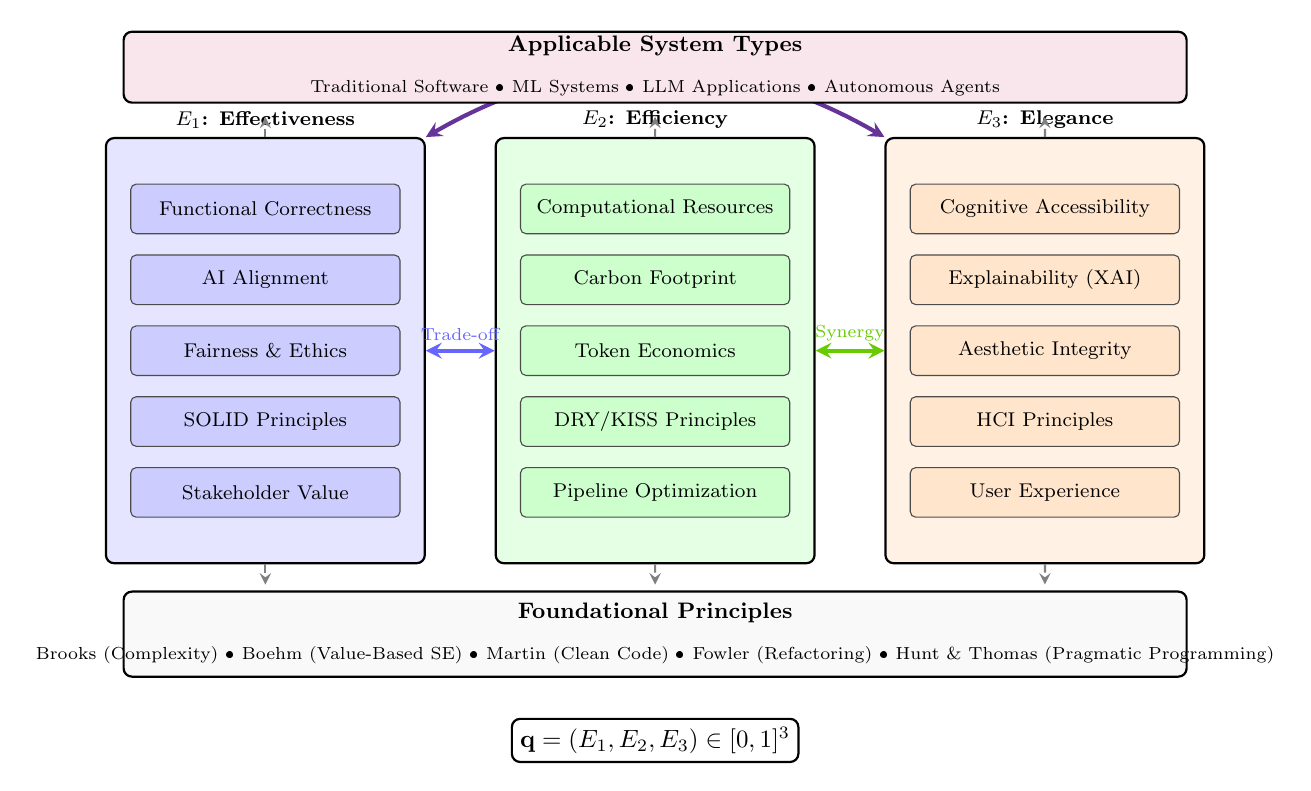
\begin{tikzpicture}[
    scale=0.9,
    transform shape,
    pillar/.style={
        rectangle,
        draw=black,
        thick,
        rounded corners=3pt,
        minimum width=4.5cm,
        minimum height=6cm,
        align=center,
        font=\small
    },
    component/.style={
        rectangle,
        draw=black!70,
        fill=white,
        rounded corners=2pt,
        minimum width=3.8cm,
        minimum height=0.7cm,
        align=center,
        font=\footnotesize
    },
    principle/.style={
        rectangle,
        draw=black!50,
        fill=gray!10,
        rounded corners=2pt,
        minimum width=3.5cm,
        minimum height=0.6cm,
        align=center,
        font=\scriptsize
    },
    arrow/.style={
        ->,
        thick,
        >=stealth
    },
    doublearrow/.style={
        <->,
        thick,
        >=stealth
    },
    label/.style={
        font=\footnotesize\bfseries
    }
]

% --- E1: Effectiveness Pillar ---
\node[pillar, fill=blue!10] (e1) at (0,0) {};
\node[label, above] at (e1.north) {$E_1$: Effectiveness};
\node[component, fill=blue!20] at (0,2) {Functional Correctness};
\node[component, fill=blue!20] at (0,1) {AI Alignment};
\node[component, fill=blue!20] at (0,0) {Fairness \& Ethics};
\node[component, fill=blue!20] at (0,-1) {SOLID Principles};
\node[component, fill=blue!20] at (0,-2) {Stakeholder Value};

% --- E2: Efficiency Pillar ---
\node[pillar, fill=green!10] (e2) at (5.5,0) {};
\node[label, above] at (e2.north) {$E_2$: Efficiency};
\node[component, fill=green!20] at (5.5,2) {Computational Resources};
\node[component, fill=green!20] at (5.5,1) {Carbon Footprint};
\node[component, fill=green!20] at (5.5,0) {Token Economics};
\node[component, fill=green!20] at (5.5,-1) {DRY/KISS Principles};
\node[component, fill=green!20] at (5.5,-2) {Pipeline Optimization};

% --- E3: Elegance Pillar ---
\node[pillar, fill=orange!10] (e3) at (11,0) {};
\node[label, above] at (e3.north) {$E_3$: Elegance};
\node[component, fill=orange!20] at (11,2) {Cognitive Accessibility};
\node[component, fill=orange!20] at (11,1) {Explainability (XAI)};
\node[component, fill=orange!20] at (11,0) {Aesthetic Integrity};
\node[component, fill=orange!20] at (11,-1) {HCI Principles};
\node[component, fill=orange!20] at (11,-2) {User Experience};

% --- Trade-off Arrows ---
\draw[doublearrow, blue!60, line width=1.5pt] (e1.east) -- (e2.west) 
    node[midway, above, font=\scriptsize] {Trade-off};
\draw[doublearrow, green!60!orange, line width=1.5pt] (e2.east) -- (e3.west) 
    node[midway, above, font=\scriptsize] {Synergy};
\draw[doublearrow, blue!60!orange, line width=1.5pt, bend left=30] (e1.north east) to 
    node[midway, above, font=\scriptsize] {Trade-off} (e3.north west);

% --- Foundation Layer ---
\node[rectangle, draw=black, thick, fill=gray!5, minimum width=15cm, minimum height=1.2cm, rounded corners=3pt] (foundation) at (5.5,-4) {};
\node[font=\small\bfseries] at (5.5,-3.7) {Foundational Principles};
\node[font=\scriptsize] at (5.5,-4.3) {Brooks (Complexity) • Boehm (Value-Based SE) • Martin (Clean Code) • Fowler (Refactoring) • Hunt \& Thomas (Pragmatic Programming)};

% --- System Types (Top) ---
\node[rectangle, draw=black, thick, fill=purple!10, minimum width=15cm, minimum height=1cm, rounded corners=3pt] (systems) at (5.5,4) {};
\node[font=\small\bfseries] at (5.5,4.3) {Applicable System Types};
\node[font=\scriptsize] at (5.5,3.7) {Traditional Software • ML Systems • LLM Applications • Autonomous Agents};

% --- Connecting lines to foundation and systems ---
\draw[arrow, gray, dashed] (e1.south) -- (0,-3.3);
\draw[arrow, gray, dashed] (e2.south) -- (5.5,-3.3);
\draw[arrow, gray, dashed] (e3.south) -- (11,-3.3);
\draw[arrow, gray, dashed] (e1.north) -- (0,3.3);
\draw[arrow, gray, dashed] (e2.north) -- (5.5,3.3);
\draw[arrow, gray, dashed] (e3.north) -- (11,3.3);

% --- Quality Vector Notation ---
\node[rectangle, draw=black, thick, fill=white, rounded corners=3pt, minimum width=4cm] at (5.5,-5.5) {
    $\mathbf{q} = (E_1, E_2, E_3) \in [0,1]^3$
};

\end{tikzpicture}
\caption{The E3 Framework Architecture. Three mutually reinforcing pillars—Effectiveness ($E_1$), Efficiency ($E_2$), and Elegance ($E_3$)—provide a comprehensive quality model applicable across deterministic and probabilistic software systems. Dashed arrows indicate grounding in foundational software engineering principles; bidirectional solid arrows indicate trade-off relationships between pillars.}
\label{fig:e3_framework}
\end{figure*}

\subsection{Effectiveness: SOLID Principles, User Alignment, and AI Ethics}

\subsubsection{Traditional Foundations}

Effectiveness, in its classical sense, measures the degree to which software fulfills its specified requirements. Martin's SOLID principles \cite{martin2017clean} provide the architectural foundation for effectiveness:

\begin{itemize}[leftmargin=2em]
    \item \textbf{Single Responsibility Principle (SRP):} Each module should have one reason to change. In ML systems, this translates to clear separation between data ingestion, feature engineering, model training, and inference components.
    \item \textbf{Open/Closed Principle (OCP):} Software entities should be open for extension but closed for modification. For ML pipelines, this implies designing feature transformers and model architectures that can be extended without modifying existing code.
    \item \textbf{Liskov Substitution Principle (LSP):} Subtypes must be substitutable for their base types. This principle guides the design of model interfaces, ensuring that different models can be swapped without breaking downstream consumers.
    \item \textbf{Interface Segregation Principle (ISP):} Clients should not depend on interfaces they do not use. For ML systems, this suggests separate interfaces for training, prediction, and evaluation.
    \item \textbf{Dependency Inversion Principle (DIP):} High-level modules should not depend on low-level modules; both should depend on abstractions. This enables dependency injection for model implementations and data sources.
\end{itemize}

Boehm's value-based software engineering \cite{boehm2006value} extends these structural principles by emphasizing that effectiveness must be evaluated in terms of stakeholder value. A technically correct system that does not address real user needs fails the effectiveness criterion.

\subsubsection{Extension to AI Alignment and Ethics}

In probabilistic systems, effectiveness must expand beyond functional correctness to encompass \emph{alignment}---the assurance that AI behavior reflects human intent and values. Russell \cite{russell2019human} argues that the alignment problem is the central challenge of AI development: systems may optimize for proxy objectives that diverge from what humans actually want.

E3 operationalizes alignment through several mechanisms:

\textbf{Explicit Objective Specification.} Teams must document the true objective of an AI system, distinguishing between proxy metrics (click-through rate, engagement time) and genuine goals (user satisfaction, ethical content consumption). This documentation should be revisited throughout development.

\textbf{Fairness Metrics.} Effectiveness includes fairness across demographic groups. E3 recommends defining fairness constraints during requirements gathering: demographic parity, equalized odds, calibration, or other appropriate metrics \cite{mitchell2019model}. These metrics should be monitored continuously in production.

\textbf{Bias Audits.} Regular audits should assess whether the system exhibits discriminatory behavior. This includes analyzing training data for historical bias, testing model outputs across subgroups, and monitoring for emergent bias in production.


\textbf{Transparency Requirements.} Following Gebru et al.'s Datasheets for Datasets \cite{gebru2021datasheets} and Mitchell et al.'s Model Cards \cite{mitchell2019model}, E3 requires documentation of data provenance, model capabilities, limitations, and performance across different contexts. The IEEE 7000-2021 standard \cite{ieee7000:2021} provides a process for integrating these ethical considerations throughout development.

\textbf{Human Oversight.} Critical AI decisions should include human review, particularly in high-stakes domains. E3 recommends implementing escalation mechanisms when model confidence falls below thresholds or when outputs fall outside training distribution.

\subsection{Efficiency: DRY/KISS Principles, Computational Sustainability, and MLOps}

\subsubsection{Traditional Foundations}

The efficiency pillar draws on two foundational principles from the pragmatic programming tradition. Hunt and Thomas's DRY principle \cite{hunt1999pragmatic} holds that every piece of knowledge should have a single, authoritative representation. DRY eliminates redundancy that creates maintenance burden and inconsistency risk. The KISS principle advocates for simplicity, recognizing that complex solutions introduce more opportunities for failure.

Knuth's discipline of optimization \cite{knuth1974structured} provides nuance: premature micro-optimization is counterproductive, but efficiency in critical paths deserves careful attention. The Pareto principle applies: 80\% of execution time typically occurs in 20\% of code. Identifying and optimizing these critical paths yields the greatest efficiency gains.

\subsubsection{Extension to Computational Sustainability}

The efficiency calculus changes dramatically when training a single model can emit as much carbon as five automobiles over their lifetimes \cite{strubell2019energy}. Patterson et al. \cite{patterson2021carbon} demonstrated that architecture choice, data-center energy mix, and hardware utilization can vary carbon emissions by orders of magnitude for equivalent model quality. E3 extends efficiency beyond traditional metrics to encompass \emph{computational sustainability}.

\textbf{Carbon-Aware Development.} Teams should estimate and track the carbon footprint of model training and inference. This includes selecting energy-efficient architectures, utilizing renewable energy sources, and considering model size as a constraint during design.

\textbf{Resource Optimization.} For inference-time systems, efficiency manifests as token economics. Every token sent to a large language model incurs computational cost, latency, and environmental impact. Liu et al.'s research \cite{liu2023lost} demonstrates that longer prompts can be less effective, not merely more expensive.

\textbf{Pipeline Efficiency.} Following Sculley et al.'s analysis \cite{sculley2015hidden}, E3 addresses the ``pipeline jungle'' problem. ML pipelines should be designed with the same modularity principles as traditional software: clear interfaces between stages, minimal data transformation overhead, and elimination of redundant computation.

\subsubsection{MLOps Integration}

E3 integrates with MLOps practices \cite{sridhar2022mlops} while extending them with quality metrics:

\begin{itemize}[leftmargin=2em]
    \item \textbf{Experiment Tracking:} Systematic recording of hyperparameters, metrics, and artifacts for reproducibility.
    \item \textbf{Model Versioning:} Treating models as first-class versioned artifacts with clear lineage.
    \item \textbf{Automated Retraining:} Pipelines that detect drift and trigger retraining with appropriate safeguards.
    \item \textbf{Cost Monitoring:} Tracking inference costs, latency distributions, and resource utilization.
\end{itemize}


\subsection{Elegance: HCI, UI/UX, and Cognitive Ergonomics for AI Outputs}

\subsubsection{Traditional Foundations}

The elegance pillar synthesizes human-computer interaction research with software engineering principles. Norman's \emph{The Design of Everyday Things} \cite{norman2013design} established that good design makes the system's conceptual model transparent to users. His principles remain foundational:

\begin{itemize}[leftmargin=2em]
    \item \textbf{Affordances:} The system should clearly indicate what actions are possible.
    \item \textbf{Signifiers:} Visual or auditory cues should communicate where actions can occur.
    \item \textbf{Feedback:} The system should immediately acknowledge user actions and communicate internal state.
    \item \textbf{Mapping:} Controls should map naturally to their effects.
    \item \textbf{Constraints:} The system should restrict interactions to prevent errors.
\end{itemize}

Miller's research on cognitive limits \cite{miller1956magical} provides the scientific foundation for information chunking. Human working memory can hold approximately seven (plus or minus two) chunks simultaneously. Elegant interfaces respect this constraint by organizing information into digestible units.

Nielsen's usability heuristics \cite{nielsen1994enhancing} operationalize these principles into actionable guidelines: visibility of system status, match with the real world, user control and freedom, consistency and standards, error prevention, recognition over recall, flexibility and efficiency, aesthetic and minimalist design, error recovery, and help documentation.

\subsubsection{Extension to Cognitive Ergonomics for AI}

AI systems introduce unique challenges for cognitive ergonomics. A model that produces accurate predictions but offers no insight into its reasoning violates the user's need for a coherent conceptual model. Ribeiro et al.'s LIME framework \cite{ribeiro2016should} demonstrated that locally interpretable explanations can substantially increase user trust and enable effective error correction.

E3 extends elegance to AI outputs through several mechanisms:

\textbf{Explainability by Design.} Systems should be designed with explanation mechanisms from the outset, not retrofitted. This includes selecting interpretable models where appropriate, implementing explanation techniques (LIME, SHAP, attention visualization), and designing interfaces that surface explanations appropriately.

\textbf{Confidence Communication.} AI outputs should include calibrated confidence indicators. Users should understand when a system is confident in its output and when it is uncertain. Overconfident systems undermine trust; underconfident systems reduce utility.

\textbf{Graceful Degradation.} Systems should behave sensibly when operating outside their training distribution. Rather than generating confidently wrong outputs, elegant AI systems signal uncertainty or request clarification.

\textbf{Output Formatting.} AI-generated content should respect cognitive limits. Long-form outputs should be structured with clear sections, progressive disclosure, and appropriate summarization. Information density should match user expertise.

\textbf{Interaction Patterns.} AI interfaces should support iterative refinement, allowing users to provide feedback on outputs and guide subsequent generations. This creates a collaborative dynamic rather than a one-shot query-response pattern.

% ============================================================
% 5. METRICS OPERATIONALIZATION
% ============================================================
% ============================================================
% METRICS OPERATIONALIZATION
% ============================================================

\section{Metrics Operationalization}
\label{sec:metrics_operationalization}

This section operationalizes the E3 Framework by defining specific, measurable metrics for each pillar. Each metric includes a formal definition, measurement formula, target thresholds, and data collection methodology. These metrics enable teams to quantify quality and track improvements over time.

\subsection{Metrics Framework Overview}

The E3 metrics framework follows three principles:

\begin{enumerate}[leftmargin=2em]
    \item \textbf{Measurability:} Each metric can be quantified through automated or semi-automated means.
    \item \textbf{Actionability:} Metrics inform specific engineering decisions and improvements.
    \item \textbf{Context-sensitivity:} Target thresholds adapt to domain requirements and constraints.
\end{enumerate}

\subsection{Effectiveness Metrics (\texorpdfstring{$E_1$}{E1})}

This section defines metrics for the Effectiveness pillar, encompassing functional correctness, AI alignment, and fairness. Each metric includes a formal definition, measurement formula, target threshold, and collection methodology.

\subsubsection{Functional Correctness Metrics}

\begin{table}[!htbp]
\centering
\caption{Functional Correctness Metrics}
\label{tab:functional_metrics}
\small
\begin{tabularx}{\linewidth}{@{}l X@{}}
\toprule
\textbf{Metric} & \textbf{Specification} \\
\midrule
\textbf{Accuracy} & \\
Definition & Proportion of correct predictions across test set \\
Formula & $\text{Accuracy} = \frac{TP + TN}{TP + TN + FP + FN}$ \\
Target & $\geq 0.85$ for production systems \\
Collection & Automated evaluation on held-out test set \\
Frequency & Per-release + continuous monitoring \\
\addlinespace

\textbf{F1 Score} & \\
Definition & Harmonic mean of precision and recall \\
Formula & $F_1 = 2 \cdot \frac{\text{Precision} \cdot \text{Recall}}{\text{Precision} + \text{Recall}}$ \\
Target & $\geq 0.80$ for balanced classification \\
Collection & Automated evaluation \\
Frequency & Per-release \\
\addlinespace

\textbf{Task Completion Rate} & \\
Definition & Proportion of user tasks successfully completed \\
Formula & $\text{TCR} = \frac{\text{Completed Tasks}}{\text{Total Attempted Tasks}}$ \\
Target & $\geq 0.90$ for user-facing systems \\
Collection & User interaction logging \\
Frequency & Continuous \\
\bottomrule
\end{tabularx}
\end{table}

\subsubsection{AI Alignment Metrics}

\begin{table}[!htbp]
\centering
\caption{AI Alignment Metrics}
\label{tab:alignment_metrics}
\small
\begin{tabularx}{\linewidth}{@{}l X@{}}
\toprule
\textbf{Metric} & \textbf{Specification} \\
\midrule
\textbf{Intent Alignment Score} & \\
Definition & Degree to which outputs match user intent, evaluated by human raters \\
Formula & $\text{IAS} = \frac{1}{N}\sum_{i=1}^{N} \mathbb{1}[\text{output}_i \text{ matches intent}_i]$ \\
Target & $\geq 0.85$ for production LLM applications \\
Collection & Human evaluation on sample \\
Frequency & Per-release + random sampling in production \\
\addlinespace

\textbf{Constraint Satisfaction Rate} & \\
Definition & Proportion of outputs satisfying specified constraints \\
Formula & $\text{CSR} = \frac{\text{Outputs meeting all constraints}}{\text{Total outputs}}$ \\
Target & $\geq 0.95$ for constrained generation tasks \\
Collection & Automated constraint verification \\
Frequency & Continuous \\
\addlinespace

\textbf{Hallucination Rate} & \\
Definition & Proportion of outputs containing factually incorrect claims \\
Formula & $\text{HR} = \frac{\text{Outputs with hallucinations}}{\text{Total outputs}}$ \\
Target & $\leq 0.05$ for factual applications \\
Collection & Human evaluation + automated fact-checking \\
Frequency & Per-release + production sampling \\
\bottomrule
\end{tabularx}
\end{table}

\subsubsection{Fairness and Ethics Metrics}

\begin{table}[!htbp]
\centering
\caption{Fairness and Ethics Metrics}
\label{tab:fairness_metrics}
\small
\begin{tabularx}{\linewidth}{@{}l X@{}}
\toprule
\textbf{Metric} & \textbf{Specification} \\
\midrule
\textbf{Demographic Parity Difference} & \\
Definition & Difference in positive prediction rates across groups \\
Formula & $|\Pr(\hat{Y}=1|A=0) - \Pr(\hat{Y}=1|A=1)|$ \\
Target & $\leq 0.10$ (domain-adjustable) \\
Collection & Automated evaluation on demographic data \\
Frequency & Per-release + continuous monitoring \\
\addlinespace

\textbf{Equalized Odds Difference} & \\
Definition & Difference in true positive and false positive rates across groups \\
Formula & $\max(|TPR_{A=0} - TPR_{A=1}|, |FPR_{A=0} - FPR_{A=1}|)$ \\
Target & $\leq 0.10$ \\
Collection & Automated evaluation \\
Frequency & Per-release \\
\addlinespace

\textbf{Ethical Compliance Score} & \\
Definition & Aggregate score of adherence to ethical guidelines \\
Formula & $ECS = \frac{1}{K}\sum_{k=1}^{K} c_k$ where $c_k \in \{0,1\}$ for each compliance check \\
Target & $= 1.0$ (full compliance required) \\
Collection & Checklist-based audit \\
Frequency & Per-release + annual review \\
\bottomrule
\end{tabularx}
\end{table}

\subsection{Efficiency Metrics (\texorpdfstring{$E_2$}{E2})}

This section defines metrics for the Efficiency pillar, encompassing computational resources, environmental sustainability, and token economics for LLM applications. These metrics enable teams to optimize resource utilization while maintaining quality standards.

\subsubsection{Computational Resource Metrics}

\begin{table}[!htbp]
\centering
\caption{Computational Resource Metrics}
\label{tab:compute_metrics}
\small
\begin{tabularx}{\linewidth}{@{}l X@{}}
\toprule
\textbf{Metric} & \textbf{Specification} \\
\midrule
\textbf{Inference Latency} & \\
Definition & Time to produce output for a single request \\
Formula & $L = t_{\text{response}} - t_{\text{request}}$ \\
Target & $p_{95} \leq 200\text{ms}$ for interactive, $\leq 1\text{s}$ for batch \\
Collection & Automated logging \\
Frequency & Continuous \\
\addlinespace

\textbf{Throughput} & \\
Definition & Number of requests processed per unit time \\
Formula & $T = \frac{\text{Requests}}{\text{Time Interval}}$ \\
Target & Domain-specific (e.g., $\geq 1000$ req/s for high-volume) \\
Collection & Automated logging \\
Frequency & Continuous \\
\addlinespace

\textbf{Memory Utilization} & \\
Definition & Peak memory consumption during inference \\
Formula & $M_{\text{peak}} = \max(M_t)$ over time window \\
Target & $\leq 80\%$ of allocated resources \\
Collection & System monitoring \\
Frequency & Continuous \\
\addlinespace

\textbf{FLOPs per Inference} & \\
Definition & Floating-point operations required for single inference \\
Formula & Count of multiply-add operations in forward pass \\
Target & Minimize subject to accuracy constraints \\
Collection & Model profiling \\
Frequency & Per-model-version \\
\bottomrule
\end{tabularx}
\end{table}

\subsubsection{Environmental Sustainability Metrics}

\begin{table}[!htbp]
\centering
\caption{Environmental Sustainability Metrics}
\label{tab:sustainability_metrics}
\small
\begin{tabularx}{\linewidth}{@{}l X@{}}
\toprule
\textbf{Metric} & \textbf{Specification} \\
\midrule
\textbf{Carbon Emissions (Training)} & \\
Definition & kg CO$_2$ equivalent emitted during model training \\
Formula & $C_{\text{train}} = P \cdot T \cdot CI$ where $P$ = power (kW), $T$ = time (h), $CI$ = carbon intensity \\
Target & Minimize; document and offset \\
Collection & Energy monitoring + carbon calculator \\
Frequency & Per training run \\
\addlinespace

\textbf{Carbon Emissions (Inference)} & \\
Definition & kg CO$_2$ equivalent per 1000 inferences \\
Formula & $C_{\text{infer}} = \frac{P_{\text{infer}} \cdot CI}{\text{Throughput}}$ \\
Target & $\leq 0.001$ kg CO$_2$e per 1000 inferences \\
Collection & Energy monitoring \\
Frequency & Continuous \\
\addlinespace

\textbf{Energy Efficiency Ratio} & \\
Definition & Useful output per unit energy consumed \\
Formula & $EER = \frac{\text{Quality Score}}{\text{Energy (kWh)}}$ \\
Target & Maximize; track improvements over time \\
Collection & Quality metrics + energy monitoring \\
Frequency & Per-release \\
\bottomrule
\end{tabularx}
\end{table}

\subsubsection{Token Economics Metrics (LLM-specific)}

\begin{table}[!htbp]
\centering
\caption{Token Economics Metrics}
\label{tab:token_metrics}
\small
\begin{tabularx}{\linewidth}{@{}l X@{}}
\toprule
\textbf{Metric} & \textbf{Specification} \\
\midrule
\textbf{Tokens per Query} & \\
Definition & Average total tokens (prompt + completion) per request \\
Formula & $TPQ = \frac{1}{N}\sum_{i=1}^{N}(tokens_{prompt,i} + tokens_{completion,i})$ \\
Target & Minimize while maintaining quality \\
Collection & API logging \\
Frequency & Continuous \\
\addlinespace

\textbf{Cost per Successful Interaction} & \\
Definition & Monetary cost per successfully completed user interaction \\
Formula & $CPSI = \frac{\text{Total API Cost}}{\text{Successful Interactions}}$ \\
Target & Domain-specific; track over time \\
Collection & Cost tracking + interaction logging \\
Frequency & Weekly aggregation \\
\addlinespace

\textbf{Retry Rate} & \\
Definition & Proportion of requests requiring regeneration \\
Formula & $RR = \frac{\text{Regeneration Requests}}{\text{Total Requests}}$ \\
Target & $\leq 0.10$ \\
Collection & User interaction logging \\
Frequency & Continuous \\
\addlinespace

\textbf{Quality per Token} & \\
Definition & Effectiveness score normalized by token count \\
Formula & $QPT = \frac{\text{Effectiveness Score}}{\text{Total Tokens}} \times 1000$ \\
Target & Maximize \\
Collection & Quality evaluation + token logging \\
Frequency & Per-release \\
\bottomrule
\end{tabularx}
\end{table}

\subsection{Elegance Metrics (\texorpdfstring{$E_3$}{E3})}

This section defines metrics for the Elegance pillar, encompassing usability, explainability, and output quality. These metrics ensure that AI systems are not only functional and efficient but also cognitively accessible and transparent to users.

\subsubsection{Usability Metrics}

\begin{table}[!htbp]
\centering
\caption{Usability Metrics}
\label{tab:usability_metrics}
\small
\begin{tabularx}{\linewidth}{@{}l X@{}}
\toprule
\textbf{Metric} & \textbf{Specification} \\
\midrule
\textbf{System Usability Scale (SUS)} & \\
Definition & Standardized usability questionnaire score \\
Formula & $SUS = \sum_{i=1}^{10} s_i \times 2.5$ (standard calculation) \\
Target & $\geq 68$ (above average); $\geq 80$ for excellent \\
Collection & User survey \\
Frequency & Per-release + quarterly \\
\addlinespace

\textbf{Task Completion Time} & \\
Definition & Time required for users to complete standard tasks \\
Formula & $TCT = \text{median}(t_{\text{completion}} - t_{\text{start}})$ \\
Target & Within 20\% of expert baseline \\
Collection & User interaction logging \\
Frequency & Continuous \\
\addlinespace

\textbf{Error Recovery Rate} & \\
Definition & Proportion of user errors successfully recovered \\
Formula & $ERR = \frac{\text{Recovered Errors}}{\text{Total Errors}}$ \\
Target & $\geq 0.90$ \\
Collection & User interaction logging \\
Frequency & Continuous \\
\addlinespace

\textbf{Cognitive Load Score} & \\
Definition & Subjective rating of mental effort required \\
Formula & NASA-TLX or simplified scale (1-7) \\
Target & $\leq 4$ (moderate or below) \\
Collection & User survey \\
Frequency & Per-release \\
\bottomrule
\end{tabularx}
\end{table}

\subsubsection{Explainability Metrics}

\begin{table}[!htbp]
\centering
\caption{Explainability Metrics}
\label{tab:explainability_metrics}
\small
\begin{tabularx}{\linewidth}{@{}l X@{}}
\toprule
\textbf{Metric} & \textbf{Specification} \\
\midrule
\textbf{Explanation Coverage} & \\
Definition & Proportion of outputs accompanied by explanations \\
Formula & $EC = \frac{\text{Outputs with Explanations}}{\text{Total Outputs}}$ \\
Target & $= 1.0$ for high-stakes; $\geq 0.80$ for general \\
Collection & System logging \\
Frequency & Continuous \\
\addlinespace

\textbf{Explanation Comprehensibility} & \\
Definition & User rating of how understandable explanations are \\
Formula & Mean rating on 1-5 scale from user survey \\
Target & $\geq 4.0$ \\
Collection & User survey \\
Frequency & Per-release \\
\addlinespace

\textbf{Explanation Actionability} & \\
Definition & Proportion of explanations leading to successful user action \\
Formula & $EA = \frac{\text{Actions Taken Based on Explanation}}{\text{Explanations Provided}}$ \\
Target & $\geq 0.70$ \\
Collection & User interaction logging \\
Frequency & Continuous \\
\addlinespace

\textbf{Trust Score} & \\
Definition & User self-reported trust in system outputs \\
Formula & Mean rating on validated trust scale (1-7) \\
Target & $\geq 5.0$ \\
Collection & User survey \\
Frequency & Quarterly \\
\bottomrule
\end{tabularx}
\end{table}

\subsubsection{Output Quality Metrics}

\begin{table}[!htbp]
\centering
\caption{Output Quality Metrics}
\label{tab:output_quality_metrics}
\small
\begin{tabularx}{\linewidth}{@{}l X@{}}
\toprule
\textbf{Metric} & \textbf{Specification} \\
\midrule
\textbf{Output Coherence} & \\
Definition & Rating of logical consistency and flow in generated content \\
Formula & Mean human rating on 1-5 scale \\
Target & $\geq 4.0$ \\
Collection & Human evaluation on sample \\
Frequency & Per-release \\
\addlinespace

\textbf{Format Compliance} & \\
Definition & Proportion of outputs matching specified format \\
Formula & $FC = \frac{\text{Correctly Formatted Outputs}}{\text{Total Outputs}}$ \\
Target & $\geq 0.95$ \\
Collection & Automated format verification \\
Frequency & Continuous \\
\addlinespace

\textbf{Information Density} & \\
Definition & Ratio of useful information to total output length \\
Formula & $ID = \frac{\text{Information Units}}{\text{Word Count}}$ \\
Target & Domain-specific; optimize for clarity \\
Collection & Human evaluation \\
Frequency & Per-release \\
\bottomrule
\end{tabularx}
\end{table}

\subsection{Integrated Quality Score}

The E3 Framework provides an integrated quality score that combines metrics across all three pillars:

\begin{equation}
T(\mathbf{q}) = w_1 E_1 + w_2 E_2 + w_3 E_3
\end{equation}

where each pillar score is computed as a weighted aggregate of its component metrics:

\begin{align}
E_1 &= \alpha_1 \cdot \text{Functional} + \alpha_2 \cdot \text{Alignment} + \alpha_3 \cdot \text{Fairness} \\
E_2 &= \beta_1 \cdot \text{Compute} + \beta_2 \cdot \text{Sustainability} + \beta_3 \cdot \text{TokenEcon} \\
E_3 &= \gamma_1 \cdot \text{Usability} + \gamma_2 \cdot \text{Explainability} + \gamma_3 \cdot \text{OutputQuality}
\end{align}

\subsection{Metrics Collection Infrastructure}

Implementing E3 metrics requires appropriate infrastructure:

\begin{itemize}[leftmargin=2em]
    \item \textbf{Automated Collection:} CI/CD pipeline integration for per-release metrics
    \item \textbf{Continuous Monitoring:} Real-time dashboards for production metrics
    \item \textbf{Human Evaluation:} Structured protocols for subjective metrics
    \item \textbf{Data Governance:} Privacy-preserving collection and storage
\end{itemize}

Table~\ref{tab:metrics_summary} provides a comprehensive summary of all E3 metrics.

\begin{table*}[t]
\centering
\caption{E3 Metrics Summary}
\label{tab:metrics_summary}
\small
\begin{tabularx}{\textwidth}{@{}l l X l@{}}
\toprule
\textbf{Pillar} & \textbf{Category} & \textbf{Key Metrics} & \textbf{Collection} \\
\midrule
$E_1$: Effectiveness & Functional & Accuracy, F1, Task Completion Rate & Automated \\
& Alignment & Intent Alignment, Constraint Satisfaction, Hallucination Rate & Human + Automated \\
& Fairness & Demographic Parity, Equalized Odds, Ethical Compliance & Automated + Audit \\
\addlinespace
$E_2$: Efficiency & Compute & Latency, Throughput, Memory, FLOPs & Automated \\
& Sustainability & Carbon (Training/Inference), Energy Efficiency & Monitoring \\
& Token Economics & Tokens/Query, Cost/Success, Retry Rate, Quality/Token & API Logging \\
\addlinespace
$E_3$: Elegance & Usability & SUS, Task Time, Error Recovery, Cognitive Load & Survey + Logging \\
& Explainability & Coverage, Comprehensibility, Actionability, Trust & Survey + Logging \\
& Output Quality & Coherence, Format Compliance, Information Density & Human + Automated \\
\bottomrule
\end{tabularx}
\end{table*}

This operationalization enables teams to measure, track, and improve software quality across all three E3 pillars, providing the quantitative foundation for evidence-based engineering decisions.

% ============================================================
% 6. E3 FOR PROMPT ENGINEERING
% ============================================================
\section{E3 for Prompt Engineering}

Prompt engineering has emerged as a distinct discipline at the intersection of software engineering, linguistics, and cognitive science \cite{brown2020language, wei2022chain}. The E3 Framework offers prompt engineers a structured evaluation model that balances competing concerns unique to this domain. This section adapts each pillar specifically for prompt engineering practice.

\subsection{Effectiveness in Prompts: Alignment and Accuracy}

An effective prompt produces outputs that are correct, relevant, and aligned with the user's intent. This requires clear specification of the task, desired format, and constraints---analogous to writing a precise function signature in traditional software.

\subsubsection{Task Specification}

Following Russell's alignment framework \cite{russell2019human}, prompts should make implicit assumptions explicit, reducing the probability that the model optimizes for a proxy rather than the true objective. Effective prompts specify:

\begin{itemize}[leftmargin=2em]
    \item \textbf{Role:} What perspective or expertise should the model adopt?
    \item \textbf{Task:} What specific action should the model perform?
    \item \textbf{Context:} What background information is necessary?
    \item \textbf{Constraints:} What limitations or requirements apply?
    \item \textbf{Format:} How should the output be structured?
\end{itemize}

Wei et al.'s chain-of-thought prompting \cite{wei2022chain} demonstrates that explicitly prompting for reasoning steps improves performance on complex tasks. This technique operationalizes effectiveness by ensuring the model's reasoning process aligns with the user's expectations.

\subsubsection{Alignment Mechanisms}

Prompt effectiveness must account for the alignment challenges unique to large language models. A prompt that elicits fluent, plausible-sounding outputs may fail if those outputs contain hallucinations or violate constraints. E3 recommends:

\textbf{Verification Prompts.} Include instructions for the model to verify factual claims or cite sources where applicable.

\textbf{Constraint Enforcement.} Use explicit delimiters and formatting instructions to enforce output structure.

\textbf{Negative Examples.} Specify what the model should not do, reducing the risk of undesired outputs.

\textbf{Iterative Refinement.} Design prompts as part of a conversation, allowing users to provide feedback and refine outputs.

\subsection{Efficiency in Prompts: Token Optimization and Modular Design}

Liu et al.'s findings \cite{liu2023lost} establish that prompt length is not merely a cost variable but an accuracy variable. Information placed at the beginning and end of a prompt is recalled more reliably than information buried in the middle. This discovery has profound implications for prompt efficiency.

\subsubsection{Token Economics}

At scale, prompt length translates directly into computational cost, latency, and environmental impact. Strubell et al. \cite{strubell2019energy} and Patterson et al. \cite{patterson2021carbon} demonstrated that language model inference carries significant environmental costs. E3 encourages prompt engineers to track:

\begin{itemize}[leftmargin=2em]
    \item \textbf{Tokens per Query:} Average prompt and completion length.
    \item \textbf{Output Quality per Token:} Effectiveness metrics normalized by token count.
    \item \textbf{Retry Rate:} Frequency of regeneration requests, indicating prompt inadequacy.
\end{itemize}


\subsubsection{Structural Efficiency}

Applying DRY to prompt engineering means that every sentence should carry non-redundant information. Applying KISS means favoring direct, unambiguous instructions over complex, nested conditions. Efficient prompts are \emph{front-loaded}: critical instructions and context appear first, supporting details follow, and redundant context is eliminated.

E3 recommends modular prompt design:

\begin{itemize}[leftmargin=2em]
    \item \textbf{System Prompts:} Reusable context that applies across queries.
    \item \textbf{Task Templates:} Parameterized prompts that can be instantiated for specific use cases.
    \item \textbf{Few-Shot Libraries:} Curated examples that can be included when needed.
    \item \textbf{Context Injection:} Dynamic retrieval of relevant context rather than including all possible context.
\end{itemize}

This modular approach reduces token redundancy while ensuring that necessary context is available when needed. It mirrors the modular design principles that Martin \cite{martin2017architecture} advocates for software architecture.

\subsection{Elegance in Prompts: Output Clarity and Formatting}

An elegant prompt produces outputs that are readable, well-structured, and cognitively accessible. Following Miller's chunking limits \cite{miller1956magical}, elegant prompts organize instructions into clearly delineated sections that both human reviewers and AI models can parse without ambiguity.

\subsubsection{Output Formatting}

Elegant prompts specify output format explicitly:

\begin{itemize}[leftmargin=2em]
    \item \textbf{Structure:} Use numbered lists, bullet points, or sections for complex outputs.
    \item \textbf{Length:} Specify desired length in words, sentences, or paragraphs.
    \item \textbf{Tone:} Indicate the appropriate voice (formal, conversational, technical).
    \item \textbf{Audience:} Specify the intended reader's expertise level.
\end{itemize}

\subsubsection{Readability for Developers}

Where prompts are shared across teams, elegance implies version control, peer review, and documentation---the same practices that Hunt and Thomas advocate for code \cite{hunt1999pragmatic}. Prompts should be self-documenting: their structure and intent should be apparent to developers who did not write them.

E3 recommends:

\textbf{Commentary Sections.} Include non-executed sections explaining prompt intent and design decisions.

\textbf{Consistent Conventions.} Use consistent formatting patterns (e.g., XML tags for roles, markdown for sections) across all prompts in a project.

\textbf{Changelog Documentation.} Track prompt modifications and their effects on output quality.

\textbf{Testing Protocols.} Establish evaluation suites that compare prompt versions across representative inputs.

\subsection{Balancing the Pillars in Prompt Engineering}

The three pillars may conflict in practice. A maximally efficient prompt (minimal tokens) may sacrifice effectiveness (incomplete instructions) or elegance (opaque structure). A maximally effective prompt (comprehensive instructions) may become inefficient (excessive tokens) or inelegant (difficult to parse).

E3 does not prescribe a universal weighting. Instead, it provides a vocabulary for prompt engineers to make these trade-offs explicitly:

\begin{itemize}[leftmargin=2em]
    \item For high-stakes applications (medical, legal, financial), prioritize effectiveness.
    \item For high-volume applications (customer service, content generation), prioritize efficiency.
    \item For user-facing applications (creative tools, assistants), prioritize elegance.
\end{itemize}

The framework encourages teams to define their own priorities and measure outcomes accordingly.

% ============================================================
% 7. ILLUSTRATIVE EXAMPLES
% ============================================================
% ============================================================
% ILLUSTRATIVE EXAMPLES
% ============================================================

\section{Illustrative Examples}
\label{sec:illustrative_examples}

This section presents four hypothetical scenarios demonstrating how the E3 Framework guides software quality decisions across diverse domains. Each example illustrates the application of E3 principles, trade-off analysis, and metric-driven evaluation. These scenarios are illustrative rather than empirical, designed to demonstrate framework applicability.

\subsection{Example 1: Healthcare Diagnostic AI System}

\subsubsection{Context}

A development team is building an AI system to assist radiologists in detecting early-stage lung cancer from CT scans. The system will be deployed in hospitals across diverse socioeconomic regions.

\subsubsection{E3 Analysis}

\paragraph{Effectiveness ($E_1$) Considerations}

\begin{itemize}[leftmargin=2em]
    \item \textbf{Functional Correctness:} High sensitivity required ($\geq 0.95$) to avoid missing cancers; specificity $\geq 0.90$ to minimize false positives.
    \item \textbf{AI Alignment:} System must align with clinical workflow, supporting rather than replacing radiologist judgment.
    \item \textbf{Fairness:} Model must perform equitably across demographic groups; training data must represent diverse populations.
    \item \textbf{Ethical Governance:} Compliance with medical device regulations (FDA, CE marking); clear documentation of limitations.
\end{itemize}

\paragraph{Efficiency ($E_2$) Considerations}

\begin{itemize}[leftmargin=2em]
    \item \textbf{Computational Resources:} Inference must complete within 30 seconds to integrate with clinical workflow.
    \item \textbf{Sustainability:} Training large vision models has significant carbon footprint; consider transfer learning from pre-trained models.
    \item \textbf{Cost:} Deployment cost must be sustainable for resource-constrained hospitals.
\end{itemize}

\paragraph{Elegance ($E_3$) Considerations}

\begin{itemize}[leftmargin=2em]
    \item \textbf{Explainability:} Radiologists require visual explanations (attention maps, similar cases) to trust and validate findings.
    \item \textbf{Usability:} Interface must integrate with existing PACS systems; minimal additional cognitive load.
    \item \textbf{Confidence Communication:} Clear display of uncertainty; no overconfident predictions.
\end{itemize}

\subsubsection{Trade-off Decisions}

\begin{table}[h]
\centering
\caption{Healthcare AI: E3 Trade-off Analysis}
\label{tab:healthcare_tradeoff}
\small
\begin{tabularx}{\columnwidth}{@{}l X X@{}}
\toprule
\textbf{Decision} & \textbf{Trade-off} & \textbf{E3 Resolution} \\
\midrule
Model Size & Larger model $\rightarrow$ higher accuracy but slower inference, higher cost & Prioritize $E_1$ (sensitivity); accept $E_2$ cost; optimize inference pipeline \\
Explainability & Attention maps may reduce accuracy slightly & $E_3$ is non-negotiable; accept minor $E_1$ reduction \\
Fairness & Balanced dataset may reduce overall accuracy & $E_1$ fairness component requires equitable performance \\
\bottomrule
\end{tabularx}
\end{table}

\paragraph{Weight Vector:} $\mathbf{w} = (0.55, 0.20, 0.25)$ — Effectiveness prioritized with significant elegance weight for clinical trust.

\subsubsection{Hypothetical Outcomes}

\begin{itemize}[leftmargin=2em]
    \item Sensitivity: 0.96, Specificity: 0.91 ($E_1$ = 0.88)
    \item Inference latency: 22 seconds average ($E_2$ = 0.75)
    \item SUS score: 82, Explanation comprehensibility: 4.2/5 ($E_3$ = 0.81)
    \item Integrated score: $T(\mathbf{q}) = 0.55(0.88) + 0.20(0.75) + 0.25(0.81) = 0.83$
\end{itemize}

\subsection{Example 2: Content Recommendation System}

\subsubsection{Context}

A social media platform is redesigning its content recommendation algorithm to balance engagement optimization with user well-being and content quality.

\subsubsection{E3 Analysis}

\paragraph{Effectiveness ($E_1$) Considerations}

\begin{itemize}[leftmargin=2em]
    \item \textbf{Functional:} Recommendations should match user interests while avoiding harmful content.
    \item \textbf{Alignment:} Long-term user well-being vs. short-term engagement; avoid addictive patterns.
    \item \textbf{Fairness:} Equal visibility for creators across demographic groups; avoid amplification bias.
    \item \textbf{Ethical Governance:} Transparency about recommendation criteria; user control over algorithm.
\end{itemize}

\paragraph{Efficiency ($E_2$) Considerations}

\begin{itemize}[leftmargin=2em]
    \item \textbf{Scale:} System processes millions of requests per second; latency critical.
    \item \textbf{Sustainability:} Large-scale recommendation has significant energy footprint.
    \item \textbf{Cost:} Infrastructure costs scale with model complexity.
\end{itemize}

\paragraph{Elegance ($E_3$) Considerations}

\begin{itemize}[leftmargin=2em]
    \item \textbf{Transparency:} Users should understand why content is recommended.
    \item \textbf{Control:} Users can adjust preferences, dismiss recommendations, see fewer similar items.
    \item \textbf{Aesthetic:} Clean presentation without overwhelming users.
\end{itemize}

\subsubsection{Trade-off Decisions}

\begin{table}[h]
\centering
\caption{Recommendation System: E3 Trade-off Analysis}
\label{tab:rec_tradeoff}
\small
\begin{tabularx}{\columnwidth}{@{}l X X@{}}
\toprule
\textbf{Decision} & \textbf{Trade-off} & \textbf{E3 Resolution} \\
\midrule
Engagement vs. Well-being & Pure engagement optimization harms user well-being & Redefine $E_1$ to include well-being metrics \\
Model Complexity & Deeper models improve relevance but increase latency and cost & Two-tier system: fast retrieval + slower ranking \\
Transparency & Showing reasons increases UI complexity & Progressive disclosure: explanations on hover/tap \\
\bottomrule
\end{tabularx}
\end{table}

\paragraph{Weight Vector:} $\mathbf{w} = (0.35, 0.40, 0.25)$ — Efficiency prioritized for scale, with balanced effectiveness and elegance.

\subsubsection{Hypothetical Outcomes}

\begin{itemize}[leftmargin=2em]
    \item Engagement + Well-being score: 0.78 ($E_1$ = 0.78)
    \item Latency: 45ms p95, Throughput: 50K req/s ($E_2$ = 0.85)
    \item User satisfaction with control: 3.8/5, Transparency rating: 3.9/5 ($E_3$ = 0.72)
    \item Integrated score: $T(\mathbf{q}) = 0.35(0.78) + 0.40(0.85) + 0.25(0.72) = 0.79$
\end{itemize}

\subsection{Example 3: LLM-Powered Code Assistant}

\subsubsection{Context}

A software company is developing an LLM-powered code assistant that helps developers write, review, and debug code. The assistant integrates with popular IDEs.

\subsubsection{E3 Analysis}

\paragraph{Effectiveness ($E_1$) Considerations}

\begin{itemize}[leftmargin=2em]
    \item \textbf{Functional:} Code suggestions must be syntactically correct and semantically appropriate.
    \item \textbf{Alignment:} Suggestions should match project coding standards and developer intent.
    \item \textbf{Security:} Avoid suggesting vulnerable code patterns; flag security issues.
    \item \textbf{Hallucination:} Minimize confident but incorrect suggestions.
\end{itemize}

\paragraph{Efficiency ($E_2$) Considerations}

\begin{itemize}[leftmargin=2em]
    \item \textbf{Latency:} Suggestions must appear within 200ms to maintain flow state.
    \item \textbf{Token Economics:} Optimize prompt design for quality per token.
    \item \textbf{Cost:} API costs scale with usage; balance quality and cost.
\end{itemize}

\paragraph{Elegance ($E_3$) Considerations}

\begin{itemize}[leftmargin=2em]
    \item \textbf{Integration:} Seamless IDE integration; minimal context switching.
    \item \textbf{Explanations:} When suggesting non-obvious solutions, provide brief explanations.
    \item \textbf{Progressive Disclosure:} Show suggestions unobtrusively; details on demand.
\end{itemize}

\subsubsection{Prompt Engineering Example}

\paragraph{Before E3 Optimization:}

\begin{verbatim}
User: Fix this bug

def calculate_total(items):
    total = 0
    for item in items:
        total += item.price * item.quantity
    return total
\end{verbatim}

\textit{Issues:} No context about the bug, no specification of expected behavior, no constraints on the solution.

\paragraph{After E3 Optimization:}

\begin{verbatim}
System: You are a code review assistant. Analyze code for:
- Correctness bugs (logic errors, edge cases)
- Security vulnerabilities
- Performance issues

User: Review this function for a bug where items with 
missing 'price' or 'quantity' attributes cause crashes:

def calculate_total(items):
    total = 0
    for item in items:
        total += item.price * item.quantity
    return total

Expected behavior: Skip invalid items, log warnings.
Follow PEP 8 style guidelines.
\end{verbatim}

\textit{E3 Improvements:}
\begin{itemize}[leftmargin=2em]
    \item $E_1$: Clear specification of bug type and expected behavior
    \item $E_2$: Focused prompt reduces token usage and improves relevance
    \item $E_3$: Style constraints ensure suggestions match project standards
\end{itemize}

\subsubsection{Hypothetical Outcomes}

\begin{itemize}[leftmargin=2em]
    \item Code correctness rate: 0.87, Security issue detection: 0.92 ($E_1$ = 0.85)
    \item Latency: 180ms average, Tokens/suggestion: 45 ($E_2$ = 0.80)
    \item Developer satisfaction: 4.3/5, Integration rating: 4.5/5 ($E_3$ = 0.84)
    \item Integrated score: $T(\mathbf{q}) = 0.40(0.85) + 0.30(0.80) + 0.30(0.84) = 0.83$
\end{itemize}

\subsection{Example 4: Autonomous Vehicle Decision System}

\subsubsection{Context}

An automotive company is developing the decision-making module for a Level 4 autonomous vehicle, responsible for trajectory planning and collision avoidance.

\subsubsection{E3 Analysis}

\paragraph{Effectiveness ($E_1$) Considerations}

\begin{itemize}[leftmargin=2em]
    \item \textbf{Safety:} Zero tolerance for collisions; fail-safe behavior required.
    \item \textbf{Robustness:} Must handle edge cases (weather, construction, erratic behavior).
    \item \textbf{Alignment:} Decision logic must align with ethical principles (trolley problem considerations).
    \item \textbf{Regulatory Compliance:} Meet automotive safety standards (ISO 26262).
\end{itemize}

\paragraph{Efficiency ($E_2$) Considerations}

\begin{itemize}[leftmargin=2em]
    \item \textbf{Real-time:} Decision cycle must complete within 100ms.
    \item \textbf{Hardware Constraints:} Limited compute power on vehicle; optimize for edge deployment.
    \item \textbf{Energy:} Decision system contributes to vehicle energy consumption.
\end{itemize}

\paragraph{Elegance ($E_3$) Considerations}

\begin{itemize}[leftmargin=2em]
    \item \textbf{Explainability:} Post-incident analysis requires interpretable decisions.
    \item \textbf{Passenger Communication:} Clear feedback about vehicle intentions.
    \item \textbf{Trust:} Predictable, human-like behavior patterns.
\end{itemize}

\subsubsection{Trade-off Decisions}

\begin{table}[h]
\centering
\caption{Autonomous Vehicle: E3 Trade-off Analysis}
\label{tab:av_tradeoff}
\small
\begin{tabularx}{\columnwidth}{@{}l X X@{}}
\toprule
\textbf{Decision} & \textbf{Trade-off} & \textbf{E3 Resolution} \\
\midrule
Model Complexity & Deep RL learns better policies but less interpretable & Hybrid: learned perception + rule-based safety layer \\
Latency vs. Accuracy & More computation improves accuracy but increases latency & Hardware acceleration + model optimization; $E_2$ hard constraint \\
Ethical Dilemmas & No universally correct answers & Document ethical framework; regulatory engagement \\
\bottomrule
\end{tabularx}
\end{table}

\paragraph{Weight Vector:} $\mathbf{w} = (0.60, 0.25, 0.15)$ — Effectiveness (safety) dominates; efficiency required for real-time operation.

\subsubsection{Hypothetical Outcomes}

\begin{itemize}[leftmargin=2em]
    \item Safety score: 0.99 (one intervention per 10K miles), Robustness: 0.94 ($E_1$ = 0.92)
    \item Decision latency: 78ms average, Energy efficiency: 0.82 ($E_2$ = 0.80)
    \item Explainability: 0.88 (logged decisions), Passenger trust: 4.0/5 ($E_3$ = 0.78)
    \item Integrated score: $T(\mathbf{q}) = 0.60(0.92) + 0.25(0.80) + 0.15(0.78) = 0.86$
\end{itemize}

\subsection{Cross-Example Analysis}

Table~\ref{tab:examples_comparison} compares E3 application across the four scenarios.

\begin{table*}[t]
\centering
\caption{Cross-Example Comparison of E3 Application}
\label{tab:examples_comparison}
\small
\begin{tabularx}{\textwidth}{@{}l X X X X@{}}
\toprule
\textbf{Dimension} & \textbf{Healthcare AI} & \textbf{Recommendation} & \textbf{Code Assistant} & \textbf{Autonomous Vehicle} \\
\midrule
Weight Vector & (0.55, 0.20, 0.25) & (0.35, 0.40, 0.25) & (0.40, 0.30, 0.30) & (0.60, 0.25, 0.15) \\
Primary Pillar & $E_1$ (Effectiveness) & $E_2$ (Efficiency) & Balanced & $E_1$ (Safety) \\
$E_1$ Score & 0.88 & 0.78 & 0.85 & 0.92 \\
$E_2$ Score & 0.75 & 0.85 & 0.80 & 0.80 \\
$E_3$ Score & 0.81 & 0.72 & 0.84 & 0.78 \\
Integrated T(q) & 0.83 & 0.79 & 0.83 & 0.86 \\
Key Trade-off & Accuracy vs. Speed & Engagement vs. Well-being & Quality vs. Cost & Safety vs. Interpretability \\
\addlinespace
E3 Contribution & Explicit fairness requirements; explainability for trust & Well-being in effectiveness; scale efficiency & Prompt optimization; developer experience & Safety-first weighting; ethical framework \\
\bottomrule
\end{tabularx}
\end{table*}

These examples demonstrate that:

\begin{enumerate}[leftmargin=2em]
    \item The E3 Framework adapts to diverse domains through appropriate weight vector selection.
    \item Trade-off analysis is domain-specific but follows consistent E3 principles.
    \item The integrated quality score enables comparison across systems and iterations.
    \item E3 provides vocabulary and structure for discussing quality decisions with stakeholders.
\end{enumerate}

Future empirical work should validate these hypothetical scenarios through controlled studies and real-world deployments.

% ============================================================
% 8. METHODOLOGY AND APPLICATION
% ============================================================
\section{Methodology and Application}

The E3 Framework is designed to complement rather than replace existing development methodologies. This section describes how E3 integrates with Agile, DevOps, and MLOps practices, and provides practical implementation guidelines.

\subsection{Integration with Agile Methodologies}

Agile methodologies emphasize iterative development, customer collaboration, and responding to change \cite{beck2000extreme}. E3 enhances Agile by providing explicit quality dimensions that user stories and acceptance criteria should address.

\subsubsection{User Story Enhancement}

Traditional user stories follow the format: ``As a [role], I want [feature] so that [benefit].'' E3 extends this with quality criteria:

\begin{itemize}[leftmargin=2em]
    \item \textbf{Effectiveness:} How will we verify that this story delivers genuine value?
    \item \textbf{Efficiency:} What resource constraints apply to this feature?
    \item \textbf{Elegance:} What UX/explainability requirements apply?
\end{itemize}

For AI-specific stories, additional criteria include:

\begin{itemize}[leftmargin=2em]
    \item Fairness constraints and protected attributes.
    \item Confidence thresholds for automated decisions.
    \item Explanation requirements.
    \item Human oversight triggers.
\end{itemize}

\subsubsection{Definition of Done}

E3 extends the Agile ``definition of done'' to include:

\textbf{Effectiveness:}
\begin{itemize}[leftmargin=2em]
    \item All acceptance criteria verified.
    \item Fairness metrics within acceptable bounds.
    \item Bias audit completed for AI components.
    \item Documentation complete (datasheets, model cards).
\end{itemize}

\textbf{Efficiency:}
\begin{itemize}[leftmargin=2em]
    \item Performance benchmarks met.
    \item Resource utilization within budgets.
    \item Carbon footprint estimated and acceptable.
\end{itemize}

\textbf{Elegance:}
\begin{itemize}[leftmargin=2em]
    \item UX review completed.
    \item Explainability mechanisms verified.
    \item Accessibility requirements met.
\end{itemize}

\subsection{Integration with DevOps}

DevOps practices automate the path from development to production \cite{humble2010continuous}. E3 enhances DevOps by extending CI/CD pipelines with AI-specific quality gates.

\subsubsection{Extended Pipeline Stages}

A traditional CI/CD pipeline includes stages for build, test, and deploy. E3 adds:

\textbf{Data Validation Stage:} Verify data quality, detect distribution shift, validate schema compliance.

\textbf{Model Validation Stage:} Evaluate model performance across fairness dimensions, compare against baseline, check for regression.

\textbf{Explanation Verification:} Ensure explanation mechanisms function correctly; validate that explanations are comprehensible.

\textbf{Resource Budget Check:} Verify that inference latency, memory usage, and estimated carbon impact are within bounds.


\subsubsection{Monitoring Extension}

Traditional DevOps monitoring focuses on system health (availability, latency, error rate). E3 extends monitoring to include:

\textbf{Effectiveness Monitoring:}
\begin{itemize}[leftmargin=2em]
    \item Model accuracy and drift detection.
    \item Fairness metric tracking over time.
    \item User satisfaction indicators.
    \item Alignment failure detection (outputs that violate constraints).
\end{itemize}

\textbf{Efficiency Monitoring:}
\begin{itemize}[leftmargin=2em]
    \item Inference latency distribution.
    \item Token usage and cost tracking.
    \item Resource utilization.
    \item Carbon intensity estimates.
\end{itemize}

\textbf{Elegance Monitoring:}
\begin{itemize}[leftmargin=2em]
    \item User feedback on output quality.
    \item Explanation usage patterns.
    \item Regeneration request rates.
    \item User trust indicators.
\end{itemize}

\subsection{Integration with MLOps}

MLOps extends DevOps specifically for machine learning systems \cite{sridhar2022mlops}. E3 provides MLOps with a quality framework that extends beyond operational concerns.

\subsubsection{Experiment Tracking Enhancement}

MLOps emphasizes experiment tracking for reproducibility. E3 extends this to include:

\begin{itemize}[leftmargin=2em]
    \item Fairness metrics for each experiment.
    \item Resource consumption estimates.
    \item Explanation quality evaluations.
    \item Stakeholder value alignment assessment.
\end{itemize}

\subsubsection{Model Registry Enhancement}

E3 extends model registry metadata to include:

\begin{itemize}[leftmargin=2em]
    \item Model cards with performance across demographic groups.
    \item Carbon footprint estimates for training.
    \item Inference resource requirements.
    \item Explanation mechanism specifications.
    \item Alignment documentation.
\end{itemize}

\subsubsection{Deployment Automation}

E3-informed deployment automation includes:

\textbf{Pre-deployment Checks:}
\begin{itemize}[leftmargin=2em]
    \item Bias audit verification.
    \item Fairness constraint validation.
    \item Explanation mechanism testing.
    \item Resource budget verification.
\end{itemize}

\textbf{Post-deployment Monitoring:}
\begin{itemize}[leftmargin=2em]
    \item Automated drift detection.
    \item Fairness metric alerts.
    \item User feedback collection.
    \item Cost anomaly detection.
\end{itemize}


\subsection{Implementation Checklist}

The following checklist translates E3 principles into measurable indicators organized by development stage. It is designed for teams adopting the framework for the first time.

\subsubsection{Requirements Gathering}

\begin{itemize}[leftmargin=2em]
    \item[\textbf{E1}] \textbf{Effectiveness:} Define task success criteria and fairness constraints. Identify stakeholders and ethical risks. Require datasheets for all training datasets \cite{gebru2021datasheets}.
    \item[\textbf{E2}] \textbf{Efficiency:} Establish latency, throughput, and carbon budgets. Identify critical computational paths per Knuth's principle \cite{knuth1974structured}.
    \item[\textbf{E3}] \textbf{Elegance:} Conduct user research per ISO 9241-210 \cite{iso2019ergonomics}. Define explainability requirements for AI outputs. Set cognitive-load targets informed by Miller's chunking limits \cite{miller1956magical}.
\end{itemize}

\subsubsection{Design and Architecture}

\begin{itemize}[leftmargin=2em]
    \item[\textbf{E1}] Apply SOLID principles \cite{martin2017clean} to both application logic and ML pipeline components. Ensure alignment mechanisms are architecturally explicit \cite{russell2019human}.
    \item[\textbf{E2}] Enforce DRY and orthogonality \cite{hunt1999pragmatic} across code and prompt templates. Minimize pipeline jungles \cite{sculley2015hidden}.
    \item[\textbf{E3}] Design interfaces that chunk information within Miller's limit \cite{miller1956magical}. Integrate LIME or equivalent XAI mechanisms \cite{ribeiro2016should}.
\end{itemize}

\subsubsection{Implementation and Testing}

\begin{itemize}[leftmargin=2em]
    \item[\textbf{E1}] Conduct A/B testing for effectiveness. Run bias audits against defined fairness metrics. Validate ethical compliance per IEEE 7000 \cite{ieee7000:2021}.
    \item[\textbf{E2}] Profile before optimizing. Track tokens-per-query and cost-per-inference. Benchmark against carbon budgets \cite{patterson2021carbon}.
    \item[\textbf{E3}] Perform usability testing with representative users. Validate that AI explanations are comprehensible to non-experts.
\end{itemize}

\subsubsection{Deployment and Monitoring}

\begin{itemize}[leftmargin=2em]
    \item[\textbf{E1}] Monitor user satisfaction, task completion rates, and drift in fairness metrics. Maintain a living datasheet for each deployed model.
    \item[\textbf{E2}] Track inference latency, resource utilization, and energy consumption. Alert on cost anomalies.
    \item[\textbf{E3}] Gather qualitative UX feedback. Monitor explanation quality and user trust indicators. Iterate on prompt designs based on output-quality-per-token metrics.
\end{itemize}


% ============================================================
% 9. COMPARATIVE ANALYSIS
% ============================================================
\section{Comparative Analysis}

Table~\ref{tab:comparison} positions E3 relative to three widely adopted methodologies. The comparison is not adversarial; E3 is designed to complement rather than replace these frameworks.

\begin{table*}[t]
\centering
\caption{Comparative Analysis of E3, Agile/Scrum, DevOps, and MLOps}
\label{tab:comparison}
\small
\begin{tabularx}{\textwidth}{@{}l X X X X@{}}
\toprule
\textbf{Dimension} & \textbf{E3} & \textbf{Agile/Scrum} & \textbf{DevOps} & \textbf{MLOps} \\
\midrule
\textbf{Primary Focus} & Holistic quality across effectiveness, efficiency, elegance & Iterative delivery, customer feedback & CI/CD automation, collaboration & ML model lifecycle management \\
\addlinespace
\textbf{Ethical Governance} & First-class pillar; IEEE 7000 alignment & Not explicitly addressed & Not explicitly addressed & Emerging (model cards, data sheets) \\
\addlinespace
\textbf{Sustainability Metrics} & Carbon intensity, token economics & Not addressed & Infrastructure efficiency (implicit) & Compute tracking (partial) \\
\addlinespace
\textbf{UX / Explainability} & Explicit elegance pillar; XAI integration & User stories (indirect) & Monitoring dashboards & Model monitoring (accuracy-focused) \\
\addlinespace
\textbf{Prompt Engineering} & Structured evaluation model & Not applicable & Not applicable & Emerging concern \\
\addlinespace
\textbf{Technical Debt} & Addresses via efficiency pillar & Backlog grooming (ad hoc) & Automation reduces ops debt & ML-specific debt recognized \\
\addlinespace
\textbf{Traditional SE Principles} & SOLID, DRY, KISS as foundations & Implicit & Implicit & Limited integration \\
\addlinespace
\textbf{Complementarity} & Integrates with all three & Benefits from E3 quality metrics & Benefits from E3 UX and ethics lens & Benefits from E3 sustainability KPIs \\
\bottomrule
\end{tabularx}
\end{table*}

Agile excels at adaptive planning but provides no explicit quality dimensions beyond ``working software.'' The Agile Manifesto's principle of ``working software over comprehensive documentation'' \cite{beck2000extreme} risks undervaluing the documentation that AI systems require for fairness, transparency, and accountability.

DevOps automates delivery and emphasizes collaboration between development and operations teams \cite{humble2010continuous}. However, DevOps practices were designed for deterministic services where integration tests can verify behavior. The probabilistic nature of AI outputs challenges traditional testing approaches, and DevOps is largely silent on user experience and ethical considerations.

MLOps extends DevOps for machine learning, addressing model versioning, experiment tracking, and deployment \cite{sridhar2022mlops}. While MLOps recognizes ML-specific technical debt \cite{sculley2015hidden}, it often treats fairness, explainability, and sustainability as secondary concerns---issues to be addressed if time permits rather than first-class design constraints.

E3 supplies the missing quality model---a shared vocabulary of effectiveness, efficiency, and elegance---that can be layered onto any of these process frameworks. It does not prescribe specific ceremonies or tools; instead, it provides quality criteria that existing methodologies can incorporate.


% ============================================================
% 10. THREATS TO VALIDITY
% ============================================================
% ============================================================
% THREATS TO VALIDITY
% ============================================================

\section{Threats to Validity}
\label{sec:threats_to_validity}

As a conceptual framework paper without empirical validation, this work faces several categories of validity threats. We address these transparently to guide future research and appropriate framework adoption.

\subsection{Internal Validity}

\subsubsection{Theoretical Consistency}

The E3 Framework synthesizes principles from multiple disciplines (software engineering, AI ethics, HCI, cognitive science). While this synthesis is intentional, it introduces the risk of conceptual inconsistency or category errors.

\textbf{Mitigation:} We have provided formal definitions (Section~\ref{sec:formal_definitions}) that establish precise semantics for each pillar and component. The mapping to existing quality models (Tables~\ref{tab:iso25010_comparison} and \ref{tab:mccall_comparison}) demonstrates consistency with established frameworks.

\textbf{Remaining Threat:} The boundaries between pillars may blur in practice. For example, explainability could be argued to belong to effectiveness (enabling correct use) or efficiency (reducing cognitive load) rather than elegance. We acknowledge that categorization involves judgment and encourage practitioners to adapt the framework to their context.

\subsubsection{Metric Definition Validity}

The metrics proposed in Section~\ref{sec:metrics_operationalization} operationalize abstract concepts into measurable quantities. This operationalization may not capture the full richness of the underlying concepts.

\textbf{Mitigation:} We have selected metrics with established validity (e.g., SUS for usability, demographic parity for fairness) and provided multiple metrics per concept to enable triangulation.

\textbf{Remaining Threat:} Some metrics (e.g., Intent Alignment Score) rely on human judgment, introducing subjectivity. Others (e.g., carbon footprint) depend on infrastructure-specific factors that complicate comparison. Future work should validate these metrics through inter-rater reliability studies and standardization efforts.

\subsection{External Validity}

\subsubsection{Generalizability}

The E3 Framework claims applicability across diverse system types (traditional software, ML systems, LLM applications, autonomous agents). This broad scope raises questions about whether a single framework can meaningfully address such heterogeneous domains.

\textbf{Mitigation:} The illustrative examples (Section~\ref{sec:illustrative_examples}) demonstrate framework application across four distinct domains with different weight vectors and trade-off profiles. The framework's structure—abstract pillars with domain-specific instantiations—supports adaptation.

\textbf{Remaining Threat:} The examples are hypothetical; real-world application may reveal domain-specific challenges not anticipated in our analysis. We explicitly position E3 as a ``conceptual framework'' requiring empirical validation rather than a validated methodology.

\subsubsection{Cultural and Contextual Bias}

The framework reflects perspectives primarily from Western software engineering practice and AI ethics discourse. Quality priorities and ethical norms vary across cultures and contexts.

\textbf{Mitigation:} The weight vector mechanism allows explicit customization of pillar priorities. The fairness metrics include domain-adjustable thresholds.

\textbf{Remaining Threat:} The framework's emphasis on certain values (individual autonomy, transparency) may not align with all cultural contexts. The definition of ``elegance'' may reflect aesthetic preferences not universally shared. Future work should engage diverse perspectives in framework refinement.

\subsection{Construct Validity}

\subsubsection{Completeness of Quality Dimensions}

The three-pillar structure may omit important quality dimensions not captured by Effectiveness, Efficiency, or Elegance.

\textbf{Mitigation:} The mapping to ISO 25010 (Table~\ref{tab:iso25010_comparison}) demonstrates that E3 covers all eight ISO quality characteristics, either directly or through extensions. The mapping to McCall (Table~\ref{tab:mccall_comparison}) similarly demonstrates coverage of all eleven McCall factors.

\textbf{Remaining Threat:} Quality dimensions may emerge that are not anticipated by current frameworks. For example, ``resilience to adversarial manipulation'' spans security ($E_1$) and robustness ($E_1$) but may deserve separate treatment. The framework should evolve as the field advances.

\subsubsection{Trade-off Function Validity}

The linear trade-off function $T(\mathbf{q}) = w_1 E_1 + w_2 E_2 + w_3 E_3$ assumes pillar independence and linear compensation. This may not reflect real-world quality relationships.

\textbf{Mitigation:} Proposition~\ref{prop:interdependence} explicitly identifies that pillars are not independent. The geometric mean used for $E_3$ (Definition~\ref{def:elegance}) reflects non-compensatory relationships among elegance components.

\textbf{Remaining Threat:} The actual shape of trade-off curves between pillars is unknown and likely domain-specific. Linear aggregation is a simplifying assumption that enables decision-making but may not capture threshold effects or non-linear interactions. Future empirical work should investigate actual trade-off relationships.

\subsection{Reliability}

\subsubsection{Reproducibility of Assessments}

Different teams applying the E3 Framework to the same system may produce different quality scores, particularly for subjective metrics.

\textbf{Mitigation:} We have provided specific formulas for quantitative metrics and structured protocols for human evaluation. The weight vector must be explicitly documented, enabling others to understand and critique priority decisions.

\textbf{Remaining Threat:} Without standardized tools and training, framework application may vary significantly. We recommend developing E3 assessment protocols, training materials, and potentially automated tooling to improve reliability.

\subsubsection{Framework Evolution}

As AI technology and software engineering practice evolve, the framework may require updates that complicate longitudinal comparisons.

\textbf{Mitigation:} The core pillar structure ($E_1$, $E_2$, $E_3$) is designed to be stable, while component definitions and metrics can evolve. Version control of framework specifications would enable consistent application over time.

\textbf{Remaining Threat:} Rapid AI advancement may outpace framework updates. For example, new model architectures may introduce quality concerns not currently represented.

\subsection{Ecological Validity}

\subsubsection{Laboratory vs. Real-World Application}

The illustrative examples, while detailed, remain hypothetical scenarios rather than real case studies. Framework behavior in actual development contexts may differ.

\textbf{Mitigation:} Examples are grounded in realistic domain constraints and reference actual standards (ISO 26262, FDA regulations, EU AI Act). Trade-off decisions reflect documented industry challenges.

\textbf{Remaining Threat:} Without empirical validation, confirmation that the framework improves software quality outcomes or integrates smoothly with existing development processes remains pending. The hypotheses in Section~\ref{sec:formal_definitions} provide testable predictions for future research.

\subsubsection{Practitioner Adoption Barriers}

Framework adoption faces practical barriers: learning curve, tooling requirements, organizational resistance, and integration with existing processes.

\textbf{Mitigation:} The framework is designed to complement rather than replace existing methodologies (Agile, DevOps, MLOps). Metrics can be incrementally adopted.

\textbf{Remaining Threat:} Complex frameworks often fail to achieve adoption regardless of theoretical merit. Success requires not just sound theory but effective dissemination, training, and tooling. We encourage the community to develop practical resources for E3 adoption.

\subsection{Positioning and Scope Limitations}

\subsubsection{Conceptual Framework Status}

This paper presents E3 as a conceptual framework, not a validated methodology. The distinction is important:

\begin{itemize}[leftmargin=2em]
    \item \textbf{Conceptual Framework:} Provides structure for thinking about quality; defines concepts and relationships; generates hypotheses.
    \item \textbf{Validated Methodology:} Has demonstrated effectiveness through controlled studies; provides proven procedures; has established reliability.
\end{itemize}

E3 currently occupies the former category. The testable hypotheses (H1-H4) provide a research agenda for validation.

\subsubsection{Scope Boundaries}

The framework addresses software quality for AI-enabled systems but does not cover:

\begin{itemize}[leftmargin=2em]
    \item Hardware quality considerations
    \item Data quality independent of model quality
    \item Organizational and process quality (e.g., team capability, governance structures)
    \item Business model sustainability
\end{itemize}

These scope boundaries are intentional but may limit framework applicability in contexts where these factors are critical.

\subsection{Summary of Validity Threats}

Table~\ref{tab:validity_summary} summarizes validity threats and mitigation status.

\begin{table}[h]
\centering
\caption{Summary of Validity Threats}
\label{tab:validity_summary}
\small
\begin{tabularx}{\columnwidth}{@{}l X X@{}}
\toprule
\textbf{Category} & \textbf{Key Threats} & \textbf{Mitigation Status} \\
\midrule
Internal & Conceptual consistency, metric validity & Formal definitions provided; empirical validation needed \\
External & Generalizability, cultural bias & Examples demonstrate adaptation; diverse validation needed \\
Construct & Completeness, trade-off function & ISO/McCall mapping; non-linearity acknowledged \\
Reliability & Reproducibility, evolution & Protocols specified; tooling needed \\
Ecological & Real-world application, adoption & Hypothetical examples; empirical studies needed \\
\bottomrule
\end{tabularx}
\end{table}

\subsection{Research Agenda}

To address these validity threats, the following research agenda is proposed:

\begin{enumerate}[leftmargin=2em]
    \item \textbf{Case Studies:} Apply E3 to real-world systems across domains; document challenges and adaptations.
    \item \textbf{Controlled Experiments:} Test hypotheses H1-H4 through controlled comparison of E3-guided vs. ad-hoc quality approaches.
    \item \textbf{Metric Validation:} Establish inter-rater reliability for subjective metrics; validate predictive validity against downstream outcomes.
    \item \textbf{Tool Development:} Create automated assessment tools to improve reliability and reduce adoption barriers.
    \item \textbf{Cross-Cultural Studies:} Investigate framework applicability across different cultural and organizational contexts.
    \item \textbf{Longitudinal Studies:} Track framework evolution and long-term impact on software quality outcomes.
\end{enumerate}

This transparent acknowledgment of limitations positions E3 as a contribution to ongoing discourse rather than a definitive solution. We invite the community to validate, critique, and extend the framework through empirical research.

% ============================================================
% 11. DISCUSSION AND FUTURE WORK
% ============================================================
\section{Discussion and Future Work}

\subsection{Trade-offs Between Pillars}

The E3 Framework acknowledges that balancing its three pillars involves inherent trade-offs. These tensions are not weaknesses to be eliminated but realities to be managed explicitly.

\subsubsection{Effectiveness vs. Efficiency}

A maximally effective model may require significant computational resources. State-of-the-art performance on complex tasks often demands large models with billions of parameters \cite{brown2020language}. However, the environmental and economic costs of such models may be prohibitive for many applications \cite{strubell2019energy}.

E3 encourages teams to define minimum effectiveness thresholds and then optimize efficiency, rather than pursuing maximum effectiveness at any cost. For many applications, a smaller, more efficient model that meets effectiveness criteria is preferable to a larger model that marginally exceeds them.

\subsubsection{Effectiveness vs. Elegance}

Complex models often sacrifice interpretability. Deep neural networks may achieve superior accuracy while providing little insight into their reasoning \cite{ribeiro2016should}. In high-stakes domains (healthcare, criminal justice, finance), this trade-off becomes ethically significant.

E3 requires teams to make this trade-off consciously. Where explainability is critical, teams should consider interpretable models or robust explanation mechanisms, even if this reduces raw effectiveness. The framework insists that opacity is a cost that must be justified, not an inevitable feature of AI systems.

\subsubsection{Efficiency vs. Elegance}

Elegant interfaces and comprehensive explanations require computational overhead. Generating explanations in real-time adds latency. Richly formatted outputs require additional tokens. The most efficient system would return raw predictions without explanation---but such a system would fail the elegance criterion.

E3 recommends tiered approaches: lightweight responses by default with optional detailed explanations on demand. This respects both efficiency constraints and users' need for transparency.

\subsection{Future Directions}

The E3 Framework opens several avenues for future research and development:

\subsubsection{Empirical Validation}

Rigorous empirical studies should evaluate E3's impact on software quality. Research questions include:

\begin{itemize}[leftmargin=2em]
    \item Do teams using E3 produce fairer, more sustainable, more usable AI systems?
    \item What are the costs of E3 adoption, and how do they compare to benefits?
    \item How do teams negotiate trade-offs between pillars in practice?
    \item Which E3 practices have the greatest impact on outcomes?
\end{itemize}

The testable hypotheses presented in Section~\ref{sec:formal_definitions} provide a starting point for such research.

\subsubsection{Autonomous Agents}

The rise of autonomous AI agents---systems that can plan, execute, and adapt without human intervention---presents new challenges for E3. An agent's effectiveness includes not only task completion but also safety and goal alignment over extended time horizons. Efficiency encompasses not only single-query costs but cumulative resource consumption across complex workflows. Elegance extends to how agents communicate their reasoning and seek human input.

Future work should adapt E3 for agentic systems, potentially adding new dimensions such as autonomy governance, human-AI collaboration patterns, and long-term alignment monitoring.

\subsubsection{Standardization}

The software engineering profession would benefit from standardized E3 metrics and reporting formats. Just as IEEE 7000-2021 \cite{ieee7000:2021} provides a standard process for ethical system design, future standards could define:

\begin{itemize}[leftmargin=2em]
    \item Carbon accounting methodologies for AI systems.
    \item Fairness metric reporting standards.
    \item Explainability quality criteria.
    \item Prompt engineering evaluation frameworks.
\end{itemize}

\subsubsection{Tooling Development}

Practical E3 adoption requires integrated tooling that brings together capabilities currently scattered across separate platforms:

\begin{itemize}[leftmargin=2em]
    \item Unified dashboards showing effectiveness, efficiency, and elegance metrics.
    \item Automated fairness auditing integrated into CI/CD pipelines.
    \item Carbon tracking integrated with cloud providers.
    \item Explanation quality evaluation tools.
    \item Prompt version control and testing frameworks.
\end{itemize}

\subsubsection{Education and Training}

As AI becomes integral to software development, education must evolve. E3 provides a framework for curricula that integrate traditional software engineering principles with AI-specific concerns. Future work should develop educational materials, case studies, and training programs that prepare engineers for the AI transition.


% ============================================================
% 12. CONCLUSION
% ============================================================
\section{Conclusion}

The transition from deterministic to probabilistic software systems represents the defining challenge of contemporary software engineering. Traditional methodologies---Agile, DevOps, and their descendants---provided essential guidance for deterministic systems but lack a unified quality model that spans both classical and AI-driven development.

The E3 Framework addresses this gap by extending proven software engineering principles into the AI domain. Its three pillars---Effectiveness ($E_1$), Efficiency ($E_2$), and Elegance ($E_3$)---draw on foundational work from Brooks, Boehm, Martin, Fowler, Hunt, and Thomas, while incorporating contemporary AI research on technical debt, alignment, explainability, and computational sustainability.

This paper has presented E3 as a conceptual framework with formal mathematical definitions, comparative analysis against established quality models, operationalized metrics, and illustrative examples. Transparency regarding validity threats and the need for empirical validation has been maintained throughout. The testable hypotheses proposed provide a research agenda for the community.

E3 is not a replacement for existing methodologies but a quality lens that sharpens their application to AI systems. It complements Agile with explicit quality dimensions, extends DevOps with AI-specific quality gates, and enriches MLOps with ethical, sustainability, and usability concerns.

As Brooks observed, there is no silver bullet for software complexity \cite{brooks1975mythical}. But there is value in a coherent conceptual framework that helps practitioners---whether experienced software engineers, data scientists entering production, or prompt engineers shaping AI interactions---reason about quality in a structured, measurable way. The E3 Framework provides such a framework: rigorous enough for production systems, accessible enough for newcomers, and adaptable enough to evolve with the technology it seeks to govern.

The AI transition is underway. The question is not whether software engineering will adapt, but how. The E3 Framework offers one answer: by preserving the hard-won wisdom of traditional engineering while extending it to meet the unique challenges of probabilistic, AI-driven systems. In doing so, it helps ensure that the AI systems we build are not merely powerful, but also reliable, sustainable, and humane.

% ============================================================
% REFERENCES
% ============================================================
\bibliographystyle{plain}
\bibliography{references}

\end{document}